\documentclass[a4paper]{article}

\def\npart{II}

\def\ntitle{Graph Theory}
\def\nlecturer{P.\ A.\ Russel}

\def\nterm{Michaelmas}
\def\nyear{2018}

\ifx \nauthor\undefined
  \def\nauthor{Qiangru Kuang}
\else
\fi

\ifx \ntitle\undefined
  \def\ntitle{Template}
\else
\fi

\ifx \nauthoremail\undefined
  \def\nauthoremail{qk206@cam.ac.uk}
\else
\fi

\ifx \ndate\undefined
  \def\ndate{\today}
\else
\fi

\title{\ntitle}
\author{\nauthor}
\date{\ndate}

%\usepackage{microtype}
\usepackage{mathtools}
\usepackage{amsthm}
\usepackage{stmaryrd}%symbols used so far: \mapsfrom
\usepackage{empheq}
\usepackage{amssymb}
\let\mathbbalt\mathbb
\let\pitchforkold\pitchfork
\usepackage{unicode-math}
\let\mathbb\mathbbalt%reset to original \mathbb
\let\pitchfork\pitchforkold

\usepackage{imakeidx}
\makeindex[intoc]

%to address the problem that Latin modern doesn't have unicode support for setminus
%https://tex.stackexchange.com/a/55205/26707
\AtBeginDocument{\renewcommand*{\setminus}{\mathbin{\backslash}}}
\AtBeginDocument{\renewcommand*{\models}{\vDash}}%for \vDash is same size as \vdash but orginal \models is larger
\AtBeginDocument{\let\Re\relax}
\AtBeginDocument{\let\Im\relax}
\AtBeginDocument{\DeclareMathOperator{\Re}{Re}}
\AtBeginDocument{\DeclareMathOperator{\Im}{Im}}
\AtBeginDocument{\let\div\relax}
\AtBeginDocument{\DeclareMathOperator{\div}{div}}

\usepackage{tikz}
\usetikzlibrary{automata,positioning}
\usepackage{pgfplots}
%some preset styles
\pgfplotsset{compat=1.15}
\pgfplotsset{centre/.append style={axis x line=middle, axis y line=middle, xlabel={$x$}, ylabel={$y$}, axis equal}}
\usepackage{tikz-cd}
\usepackage{graphicx}
\usepackage{newunicodechar}

\usepackage{fancyhdr}

\fancypagestyle{mypagestyle}{
    \fancyhf{}
    \lhead{\emph{\nouppercase{\leftmark}}}
    \rhead{}
    \cfoot{\thepage}
}
\pagestyle{mypagestyle}

\usepackage{titlesec}
\newcommand{\sectionbreak}{\clearpage} % clear page after each section
\usepackage[perpage]{footmisc}
\usepackage{blindtext}

%\reallywidehat
%https://tex.stackexchange.com/a/101136/26707
\usepackage{scalerel,stackengine}
\stackMath
\newcommand\reallywidehat[1]{%
\savestack{\tmpbox}{\stretchto{%
  \scaleto{%
    \scalerel*[\widthof{\ensuremath{#1}}]{\kern-.6pt\bigwedge\kern-.6pt}%
    {\rule[-\textheight/2]{1ex}{\textheight}}%WIDTH-LIMITED BIG WEDGE
  }{\textheight}% 
}{0.5ex}}%
\stackon[1pt]{#1}{\tmpbox}%
}

%\usepackage{braket}
\usepackage{thmtools}%restate theorem
\usepackage{hyperref}

% https://en.wikibooks.org/wiki/LaTeX/Hyperlinks
\hypersetup{
    %bookmarks=true,
    unicode=true,
    pdftitle={\ntitle},
    pdfauthor={\nauthor},
    pdfsubject={Mathematics},
    pdfcreator={\nauthor},
    pdfproducer={\nauthor},
    pdfkeywords={math maths \ntitle},
    colorlinks=true,
    linkcolor={red!50!black},
    citecolor={blue!50!black},
    urlcolor={blue!80!black}
}

\usepackage{cleveref}



% TODO: mdframed often gives bad breaks that cause empty lines. Would like to switch to tcolorbox.
% The current workaround is to set innerbottommargin=0pt.

%\usepackage[theorems]{tcolorbox}





\usepackage[framemethod=tikz]{mdframed}
\mdfdefinestyle{leftbar}{
  %nobreak=true, %dirty hack
  linewidth=1.5pt,
  linecolor=gray,
  hidealllines=true,
  leftline=true,
  leftmargin=0pt,
  innerleftmargin=5pt,
  innerrightmargin=10pt,
  innertopmargin=-5pt,
  % innerbottommargin=5pt, % original
  innerbottommargin=0pt, % temporary hack 
}
%\newmdtheoremenv[style=leftbar]{theorem}{Theorem}[section]
%\newmdtheoremenv[style=leftbar]{proposition}[theorem]{proposition}
%\newmdtheoremenv[style=leftbar]{lemma}[theorem]{Lemma}
%\newmdtheoremenv[style=leftbar]{corollary}[theorem]{corollary}

\newtheorem{theorem}{Theorem}[section]
\newtheorem{proposition}[theorem]{Proposition}
\newtheorem{lemma}[theorem]{Lemma}
\newtheorem{corollary}[theorem]{Corollary}
\newtheorem{axiom}[theorem]{Axiom}
\newtheorem*{axiom*}{Axiom}

\surroundwithmdframed[style=leftbar]{theorem}
\surroundwithmdframed[style=leftbar]{proposition}
\surroundwithmdframed[style=leftbar]{lemma}
\surroundwithmdframed[style=leftbar]{corollary}
\surroundwithmdframed[style=leftbar]{axiom}
\surroundwithmdframed[style=leftbar]{axiom*}

\theoremstyle{definition}

\newtheorem*{definition}{Definition}
\surroundwithmdframed[style=leftbar]{definition}

\newtheorem*{slogan}{Slogan}
\newtheorem*{eg}{Example}
\newtheorem*{ex}{Exercise}
\newtheorem*{remark}{Remark}
\newtheorem*{notation}{Notation}
\newtheorem*{convention}{Convention}
\newtheorem*{assumption}{Assumption}
\newtheorem*{question}{Question}
\newtheorem*{answer}{Answer}
\newtheorem*{note}{Note}
\newtheorem*{application}{Application}

%operator macros

%basic
\DeclareMathOperator{\lcm}{lcm}

%matrix
\DeclareMathOperator{\tr}{tr}
\DeclareMathOperator{\Tr}{Tr}
\DeclareMathOperator{\adj}{adj}

%algebra
\DeclareMathOperator{\Hom}{Hom}
\DeclareMathOperator{\End}{End}
\DeclareMathOperator{\id}{id}
\DeclareMathOperator{\im}{im}
\DeclarePairedDelimiter{\generation}{\langle}{\rangle}

%groups
\DeclareMathOperator{\sym}{Sym}
\DeclareMathOperator{\sgn}{sgn}
\DeclareMathOperator{\inn}{Inn}
\DeclareMathOperator{\aut}{Aut}
\DeclareMathOperator{\GL}{GL}
\DeclareMathOperator{\SL}{SL}
\DeclareMathOperator{\PGL}{PGL}
\DeclareMathOperator{\PSL}{PSL}
\DeclareMathOperator{\SU}{SU}
\DeclareMathOperator{\UU}{U}
\DeclareMathOperator{\SO}{SO}
\DeclareMathOperator{\OO}{O}
\DeclareMathOperator{\PSU}{PSU}

%hyperbolic
\DeclareMathOperator{\sech}{sech}

%field, galois heory
\DeclareMathOperator{\ch}{ch}
\DeclareMathOperator{\gal}{Gal}
\DeclareMathOperator{\emb}{Emb}



%ceiling and floor
%https://tex.stackexchange.com/a/118217/26707
\DeclarePairedDelimiter\ceil{\lceil}{\rceil}
\DeclarePairedDelimiter\floor{\lfloor}{\rfloor}


\DeclarePairedDelimiter{\innerproduct}{\langle}{\rangle}

%\DeclarePairedDelimiterX{\norm}[1]{\lVert}{\rVert}{#1}
\DeclarePairedDelimiter{\norm}{\lVert}{\rVert}



%Dirac notation
%TODO: rewrite for variable number of arguments
\DeclarePairedDelimiterX{\braket}[2]{\langle}{\rangle}{#1 \delimsize\vert #2}
\DeclarePairedDelimiterX{\braketthree}[3]{\langle}{\rangle}{#1 \delimsize\vert #2 \delimsize\vert #3}

\DeclarePairedDelimiter{\bra}{\langle}{\rvert}
\DeclarePairedDelimiter{\ket}{\lvert}{\rangle}




%macros

%general

%divide, not divide
\newcommand*{\divides}{\mid}
\newcommand*{\ndivides}{\nmid}
%vector, i.e. mathbf
%https://tex.stackexchange.com/a/45746/26707
\newcommand*{\V}[1]{{\ensuremath{\symbf{#1}}}}
%closure
\newcommand*{\cl}[1]{\overline{#1}}
%conjugate
\newcommand*{\conj}[1]{\overline{#1}}
%set complement
\newcommand*{\stcomp}[1]{\overline{#1}}
\newcommand*{\compose}{\circ}
\newcommand*{\nto}{\nrightarrow}
\newcommand*{\p}{\partial}
%embed
\newcommand*{\embed}{\hookrightarrow}
%surjection
\newcommand*{\surj}{\twoheadrightarrow}
%power set
\newcommand*{\powerset}{\mathcal{P}}

%matrix
\newcommand*{\matrixring}{\mathcal{M}}

%groups
\newcommand*{\normal}{\trianglelefteq}
%rings
\newcommand*{\ideal}{\trianglelefteq}

%fields
\renewcommand*{\C}{{\mathbb{C}}}
\newcommand*{\R}{{\mathbb{R}}}
\newcommand*{\Q}{{\mathbb{Q}}}
\newcommand*{\Z}{{\mathbb{Z}}}
\newcommand*{\N}{{\mathbb{N}}}
\newcommand*{\F}{{\mathbb{F}}}
%not really but I think this belongs here
\newcommand*{\A}{{\mathbb{A}}}

%asymptotic
\newcommand*{\bigO}{O}
\newcommand*{\smallo}{o}

%probability
\newcommand*{\prob}{\mathbb{P}}
\newcommand*{\E}{\mathbb{E}}

%vector calculus
\newcommand*{\gradient}{\V \nabla}
\newcommand*{\divergence}{\gradient \cdot}
\newcommand*{\curl}{\gradient \cdot}

%logic
\newcommand*{\yields}{\vdash}
\newcommand*{\nyields}{\nvdash}

%differential geometry
\renewcommand*{\H}{\mathbb{H}}
\newcommand*{\transversal}{\pitchfork}
\renewcommand{\d}{\mathrm{d}} % exterior derivative

%number theory
\newcommand*{\legendre}[2]{\genfrac{(}{)}{}{}{#1}{#2}}%Legendre symbol


\newcommand*{\Omg}{\Omega}
\newcommand*{\bigT}{\Theta}
\newcommand*{\smallomg}{\omega}
\DeclareMathOperator{\exx}{ex} % forbidden subgraph notation
\DeclareMathOperator{\ud}{ud} % upper density

\let\SO\undefined
\usepackage{tkz-graph}

\begin{document}

\begin{titlepage}
  \begin{center}
    
\includegraphics[width=0.6\textwidth]{logo.jpg}\par
    \vspace{1cm}
    {\scshape\huge Mathematics Tripos \par}
    \vspace{2cm}
    {\huge Part \npart \par}
    \vspace{0.6cm}
    {\Huge \bfseries \ntitle \par}
    \vspace{1.2cm}
    {\Large\nterm, \nyear \par}
    \vspace{2cm}
    
    {\large \emph{Lectures by } \par}
    \vspace{0.2cm}
    {\Large \scshape \nlecturer}
    
    \vspace{0.5cm}
    {\large \emph{Notes by }\par}
    \vspace{0.2cm}
    {\Large \scshape \href{mailto:\nauthoremail}{\nauthor}}
 \end{center}
\end{titlepage}

\tableofcontents

\setcounter{section}{-1}

\section{Introduction}

Informally, a \emph{graph} consists of some vertices with some pairs of ``vertices'' joined by ``edges''. (formal definition later)

A few problems:
\begin{enumerate}
\item bridges of Königsberg (Euler, 18th century): is it possible to walk round the city crossing each bridge precisely once and returing to starting point? Convert it into a graph, the question becomes: is it possible to walk round the ``graph'', traversing each edge precisely once, finishing at the starting vertex?\footnote{This is actually a multigraph, with more than one edge joining two vertices.}
\item four colour problem (first proposed in 19th century): how many colours are needed to colour a map? Denote each country by a vertex and connect two vertices by an edge if the countries are neighbours. Conjecture: let \(G\) be a graph that can be drawn in the plane with no crossings. Then the vertices of \(G\) can be coloured with \(4\) colours such that each edge has different coloured endpoints.
\item simultaneous coset representation (1930s): let \(G\) be a finite group, \(H \leq G\). Lagrange's Theorem says that \(|H| \divides |G|\) and if \(|G|/|H| = n\) then there are \(a_1, \dots, a_n \in G\) such that \(a_1H, \dots, a_nH\) are the left cosets of \(H\). Similarly there exist \(b_1, \dots, b_n \in G\) such that \(Hb_1, \dots, Hb_n\) are the right cosets. We can ask the problem: can we make the \(a_i\)'s and \(b_i\)'s the same? i.e.\ can we find \(c_1, \dots, c_n \in G\) such that the left cosets of \(H\) are \(c_1H, \dots, c_nH\) and the rights cosets are \(Hc_1, \dots, Hc_n\)? Recall that if \(L\) is a left coset of \(H\) and \(g \in G\) then \(L = gH\) if and only if \(g \in L\). Take set \(X\) of vertices, one for each left coset, disjoint set \(Y\) of vertices, one for each right coset. For each \(g \in G\), add an edge from \(gH\) to \(Hg\). The problem now becomes: can we find a set of edges meeting each vertex precisely once?
\item Fermat equation mod \(p\): Fermat asserted that \(x^n + y^n = z^n\) has no non-trivial solutions in integers if \(n \geq 3\). 

  \begin{theorem}
    Let \(n \in \N\). Then for any sufficiently large prime \(p\), there are \(x, y, z \neq 0 \pmod p\) with \(x^n + y^n = z^n \pmod p\).
  \end{theorem}

  The original proof involves lots of number theory and is hard. However we can reduce it to a graph theory problem. Let \(G = \Z_p^*\), multiplicative group of nonzero residues mod \(p\). Let \(H = \{g^n: g \in G\} \leq G\). We want \(x, y, z \in H\) with \(x + y = z\). We can check \(|H| \geq \frac{|G|}{n}\) so \(H\) has at most \(n\) left cosets. Suppose now in some left coset \(gH\) we have \(u, v, w \in gH\) with \(u + v = w\). Then \(g^{-1}u + g^{-1}v = g^{-1}w\) is a solution in \(H\). Thus we have reduced the theorem to the following combinatorial statement:

  \begin{theorem}[Schur]
    Let \(k\) be a positive integer. Then for any sufficiently large \(n\), if \([n] = \{1, 2, \dots, n\}\) is partitioned into \(k\) parts, then we can find \(x, y, z\) in the same part with \(x + y = z\).
  \end{theorem}
\end{enumerate}

Let's consider small cases to gain some intuition first. For \(k = 1\), take \(n = 2\). It is trivial.

For \(k = 2\), take \(n = 5\). Suppose \([5]\) is partitioned into \(A\) and \(B\). wlog \(|A| \geq 3\), say \(i < j < k\) in \(A\). If \(j - i \in A\) then \(i + (j - i) = j\) so done. Similarly if \(k - i \text{ or } k - j \in A\). Otherwise, \(j - i, k - j, k - i \in B\) and \((j - i) + (k - j) = k - i\) so done.

For \(k = 3\), take \(n = 16\). Suppose \([16]\) is partitioned in \(A, B\) and \(C\). wlog \(|A| \geq 6\) and \(a_1 < \dots < a_6\) in \(A\). If \(a_j - a_i \in A\) for some \(i < j\) then done. If not, consider \(a_2 - a_1, a_3 - a_1, \dots, a_6 - a_1 \in B \cup C\) so wlog have \(2 \leq i < j < k < 6\) such that \(a_i - a_1, a_j - a_1, a_k - a_1 \in B\). Now if \(a_j - a_i \text{ or } a_k - a_j \text{ or } a_k - a_i \in B\) then done. Otherwise \(a_j - a_i, a_k - a_j, a_k - a_i \in C\) and so done.

The ``if not'' part of \(k = 3\) feels quite like \(k = 2\) case, except that we are dealing with \(a_i - a_1\) instead of \(1, \dots, 5\). It is a bit tricky but we can do this by induction. This is left as an exercise.

Note that what we care is the difference between the numbers. More specifically, we only care the difference between \emph{a pair} of numbers, instead of what the actual difference is. This prompts us to rephrase this as a graph theory problem. Let \([5] = A \cup B\), say \(A = \{1, 3, 5\}, B = \{2, 4\}\). Take the graph with vertices \(0, \dots, 5\) and all possible edges. Colour the edge \(ij (i < j)\) to represent which of \(A, B\) contains \(j - i\).

\begin{center}
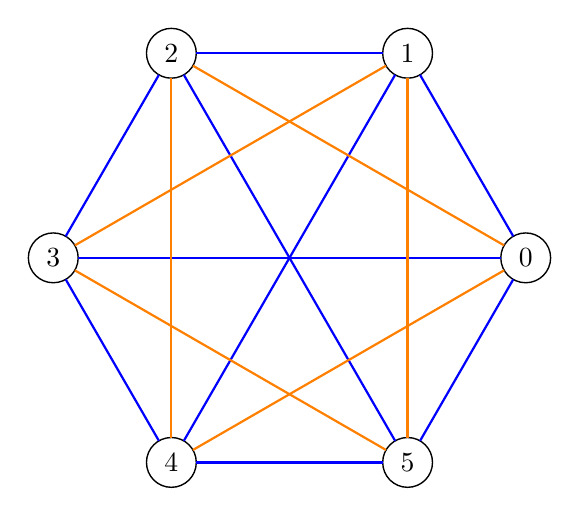
\begin{tikzpicture}
  \SetGraphUnit{3}
  \SetUpEdge[color = blue]
  \Vertices{circle}{0, 1, 2, 3, 4, 5}
  \Edges(0, 1, 2, 3, 4, 5, 0)
  \Edges(0, 3)
  \Edges(1, 4)
  \Edges(2, 5)
  \SetUpEdge[color = orange]
  \Edges(0, 2, 4, 0)
  \Edges(1, 3, 5, 1)
\end{tikzpicture}
\end{center}

Supoose we have a monochromatic triangle \(i < j < k\), then \(j - i, k - j, k - i\) are in the same part with \((k - j) + (j - i) = k - i\). This turns out to be exactly the setting we need to solve this problem. We will do this in chapter 1, alongside building the machinary we need.

\section{Extremal graph theory}

\subsection{Ramsey theory}

\begin{definition}[graph, vertex, edge]\index{graph}
  A \emph{graph} \(G\) is an ordered pair \(G = (V, E)\) where \(V\) is a finite set and \(E\) is a set of unordered pairs of distinct elements of \(V\). The elements of \(V\) are the \emph{vertices} of \(G\) and those of \(E\) the \emph{edges}. Write \(V = V(E)\) and \(E = E(G)\).
\end{definition}

\begin{eg}
  \(G = ([9], \{12, 13, 14, 23, 67, 68, 69\})\). We often use picture to represent a graph.
  \begin{center}
    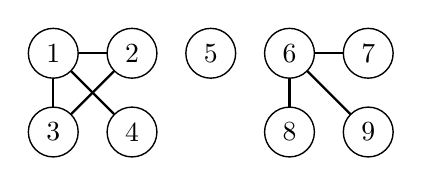
\begin{tikzpicture}
      \SetGraphUnit[3]
      \Vertex{1}
      \Vertex[x=1,y=0]{2}
      \Vertex[x=0,y=-1]{3}
      \Vertex[x=1,y=-1]{4}
      \Edges(1, 2, 3, 1)
      \Edges(1, 4)

      \Vertex[x=2,y=0]{5}

      \Vertex[x=3,y=0]{6}
      \Vertex[x=4,y=0]{7}
      \Vertex[x=3,y=-1]{8}
      \Vertex[x=4,y=-1]{9}
      \Edges(8,6,7)
      \Edges(6,9)
    \end{tikzpicture}
  \end{center}
\end{eg}

\begin{notation}
  We denote the edge \(\{i, j\}\) by \(ij\).
\end{notation}

\begin{eg}
  The \emph{complete graph of order \(n\)} \(K_n\) has \(V[K_n] = [n]\) and \(E(K_n) = \{ij: 1 \leq i < j \leq n\}\). For example, \(K_3\) is the \emph{triangle}\index{triangle}.
  \begin{center}
    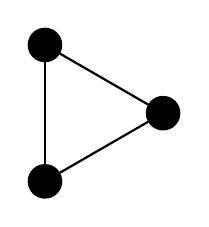
\begin{tikzpicture}
      \GraphInit[vstyle=Classic]
      \Vertices[NoLabel]{circle}{1, 2, 3}
      \Edges(1, 2, 3, 1)
    \end{tikzpicture}

    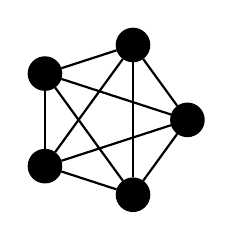
\begin{tikzpicture}
      \GraphInit[vstyle=Classic]
      \Vertices[NoLabel]{circle}{1, 2, 3, 4, 5}
      \Edges(1, 2, 3, 4, 5, 1, 3, 5, 2, 4, 1)
    \end{tikzpicture}
  \end{center}
\end{eg}

\begin{definition}[isomorphism]\index{isomorphism}
  An \emph{isomorphism} from a graph \(G\) to a graph \(H\) is a bijection \(\phi: V(G) \to V(H)\) satisfying \(\phi(u) \phi(v) \in E(H)\) if and only if \(uv \in E(G)\). If such \(\phi\) exists, we say \(G\) and \(H\) are \emph{isomorphic} and write \(G \cong H\).
\end{definition}

\begin{definition}[subgraph]\index{subgraph}
  A graph \(H\) is a \emph{subgraph} of a graph \(G\) if \(V(H) \subseteq V(G)\) and \(E(H) \subseteq E(G)\).

  More loosely, we say \(H\) is a subgraph of \(G\) if \(H \cong H'\) for some subgraph \(H'\) of \(G\).

  Write \(H \subseteq G\) to mean \(H\) is a subgraph of \(G\).
\end{definition}

\begin{notation}
  Write \(v \in G\) to mean \(v \in V(G)\).
\end{notation}

\begin{definition}[colouring]\index{colouring}
  A \emph{\(k\)-colouring} of a graph \(G\) is a function \(c: E(G) \to [k]\).
\end{definition}

In proofs, if \(K\) is small, we often call colours blue, yellow, etc.\ rather than \(1, 2, \dots\).

\begin{definition}[monochromatic]\index{monochromatic}
  If \(G\) is \(k\)-coloured and \(H \subseteq G\), we say \(H\) is \emph{monochromatic} if \(c|_{E(H)}\) is constant.
\end{definition}

Now we are ready to tackle the colouring problem in the previous chapter.

\begin{eg}
  Suppose \(K_6\) is coloured blue/yellow. Pick \(v \in K_6\). \(v\) has \(5\) edges so some \(3\) are the same colour, wlog blue \(vw, vx, vy\). If any of \(wx, wy, xy\) is blue then we have a blue triangle. Otherwise \(wxy\) is a yellow triangle. Done.
\end{eg}

\begin{note}
  Note that it doesn't work in \(K_5\), i.e.\ \(K_5\) can be \(2\)-coloured with no monochromatic triangle:
  \begin{center}
    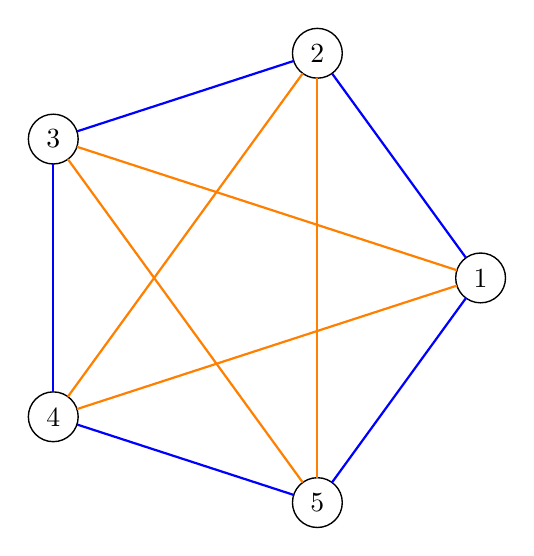
\begin{tikzpicture}
      \SetGraphUnit{3}
      \Vertices{circle}{1, 2, 3, 4, 5}
      \SetUpEdge[color = blue]
      \Edges(1,2,3,4,5,1)
      \SetUpEdge[color = orange]
      \Edges(1,3,5,2,4,1)
    \end{tikzpicture}
  \end{center}
\end{note}

\begin{proposition}[Ramsey theorem for triangles]\index{Ramsey theorem!for triangle}
  Let \(k \in \N\). Then for \(n\) sufficiently large, if \(K_n\) is \(k\)-coloured we must have a monochromatic triangle.
\end{proposition}

\begin{proof}
  Induction on \(k\). For \(k = 1\), \(n = 3\) works. For \(k > 1\), by induction hypothesis we can choose \(m\) such that if \(K_m\) is \((k - 1)\)-coloured then it has a monochromatic triangle. Now take \(n = k(m - 1) + 2\). Suppose \(K_n\) is \(k\)-coloured. Pick \(v \in K_n\). There are \(k(m - 1) + 1\) edges from \(v\) so some \(m\) are the same colour. wlog \(v\) is joint to a \(K_m\), \(H\), by blue edegs. If \(H\) contains a blue edge then we have a blue triangle with \(v\). If not then \(H\) is a \((k - 1)\)-coloured \(K_m\) so by definition of \(m\) it contains a monochromatic triangle.
\end{proof}

\begin{remark}
  How big should we take \(n\)? Write \(f(k)\) for the smallest \(n\) that works. Then \(f(1) = 3\). If \(k > 1\), the proof tells us that \(f(k) \leq k(f(k - 1) - 1) + 2 \leq k f(k - 1)\). So by induction \(f(k) \leq 3k!\).
\end{remark}

\begin{corollary}[Schur's theorem]\index{Schur's theorem}
  Let \(k \geq 1\). Then for \(n\) sufficiently larger, if \([n]\) is partitioned into \(k\) parts we can find \(x, y, z\) in the same part with \(x + y = z\).
\end{corollary}

\begin{proof}
  Let \(n\) be such that if \(K_{n + 1}\) is \(k\)-coloured then there exists a monochromatic triangle. Partition
  \[
    [n] = A_1 \cup \dots \cup A_k.
  \]
  Now \(k\)-colour a \(K_{n + 1}\) with vertices \(0, \dots, n\) using colouring \(c\), with, for \(i < j\), \(j - i \in A_{c(ij)}\). Let \(h < i < j\) be a monochormatic triangle of colour \(u\), say. Then
  \[
    (i - h) + (j - i) = j - h
  \]
  and they are all in \(A_u\).
\end{proof}

We have shown that we can always find a monochromatic triangle, i.e.\ \(K_3\). What about \(K_4, K_5\) etc?

\begin{eg}
  Suppose \(K_{10}\) is coloured blue/yellow. Then there must be a blue triangle or a yellow \(K_4\).

  \begin{proof}
    Pick \(v \in K_{10}\), then
    \begin{itemize}
    \item either \(v\) is in \(4\) blue edges \(vw, vx, vy, vz\). If any edge is among \(w, x, y, z\) is blue, we have a blue triangle. Else \(wxyz\) is a yellow \(K_4\),
      \begin{center}
      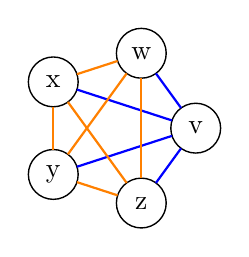
\begin{tikzpicture}
        \Vertices{circle}{v, w, x, y, z}
        \SetUpEdge[color=blue]
        \Edges(w, v, z)
        \Edges(y, v, x)
        \SetUpEdge[color=orange]
        \Edges(w, x, y, z, w, y)
        \Edges(x, z)
      \end{tikzpicture}
      \end{center}
    \item or \(v\) is in \(6\) yellow edges. Let \(H\) be a \(K_6\) joined to \(v\) by yellow edges. We know \(H\) must have a monochromatic triangle. If it is a blue done. Otherwise together with \(v\) we have a yellow \(K_4\).
    \end{itemize}
  \end{proof}
\end{eg}

\begin{definition}[Ramsey number]\index{Ramsey number}
  Let \(s, t \geq 2\). The \emph{Ramsey number} \(R(s, t)\) is the least \(n\) such that whenever \(K_n\) is coloured blue/yellow then we can find a blue \(K_s\) or a yellow \(K_t\) (if such an \(n\) exists). We write \(R(s) = R(s, s)\).
\end{definition}

\begin{theorem}[Ramsey]\index{Ramsey theorem}
  Let \(s, t \geq 2\). Then \(R(s, t)\) exists. Moreover, if \(s, t \geq 3\) then
  \[
    R(s, t) \leq R(s - 1, t) + R(s, t - 1).
  \]
\end{theorem}

\begin{proof}
  Induction on \(s + t\). For \(s = 2\), \(R(2, t) = t\) and similarly for \(t = 2\), \(R(s, 2) = s\). For \(s, t \geq 3\), by induction hypothesis we can take
  \begin{align*}
    m &= R(s - 1, t) \\
    n &= R(s, t -1)
  \end{align*}
  Colour \(K_{m + n}\) blue/yellow. Pick a vertex \(v \in K_{m + n}\). Then
  \begin{itemize}
  \item either \(v\) is in \(m\) blue edges. Let \(H\) be a \(K_m\) joined to \(v\) by blue. By definition of \(m\), \(H\) contains either a blue \(K_{s - 1}\), making a blue \(K_s\) with \(v\) or a yellow \(K_t\).
  \item or \(v\) is in \(n\) yellow edges. Proceed as before with blue/yellow reversed.
  \end{itemize}
  Hence \(R(s, t)\) exists and moreover
  \[
    R(s, t) \leq R(s- 1, t) + R(s, t - 1).
  \]
\end{proof}

How big is \(R(s)\)? We know \(R(2) = 2, R(3) = 6\) so
\[
  R(3, 4) \leq R(3) + R(2, 4) \leq 10.
\]
In fact, in example sheet we will show \(R(3, 4) = 9\). Then
\[
  R(4) = R(4, 4) \leq 2R(3, 4) = 18.
\]
It turns out to be a sharp, which we will also show on example sheet. What about \(R(5)\)? Nobody knows exactly. The bound as the time the note is taken is \(43 \leq R(5) \leq 48\). Although \(5\) seem innocuouly small, the computation required to find the exact Ramsey number is enourmous: as \(R(5) \approx 45\), \(K_{45}\) has \(\binom{45}{2} \approx 1000\) edges so there are approximately \(2^{1000}\) blue/yellow colourings.

However, we can easily bound them:

\begin{corollary}
  Let \(s, t \geq 2\). Then \(R(s, t) \leq 2^{s + t}\). In particular, \(R(s) \leq 4^s\).
\end{corollary}

\begin{proof}
  Induction on \(s + t\). For \(s = 2\) have \(R(2, t) = t \leq 2^{2 + t}\). Same for \(t = 2\). For \(s, t \geq 3\),
  \[
    R(s, t) \leq R(s - 1, t) + R(s, t - 1) \leq 2^{s - 1 + t} + 2^{s + t - 1} = 2^{s + t}.
  \]
\end{proof}

\(R(s) \leq 4^s\) seems like a rather crude bound --- indeed we start the induction with a very sloppy \(t \leq 2^t\). If we do it more carefully, we get \(R(s, t) \leq \binom{s + t - 2}{s - 1}\) so \(R(s) \leq \binom{2s - 2}{s - 1}\). Approximate, e.g.\ by Stirling formula and we get
\[
  R(s) = O(\frac{4^s}{\sqrt s}),
\]
which is the result by Erdős-Szekeres in 1930s. For 50 years no one is able to improve it. In the 1980s, Andrew Thomason shows \(R(s) = O(\frac{4^s}{s})\), which takes considerably more work. So far the best bound is found by David Conlon in the 2000s, for all \(k\), \(R(s) = O(\frac{4^s}{s^k})\). Is \(R(s) = O((4 - \varepsilon)^s)\) for some \(\varepsilon > 0\)? The answer is unknown.

For a lower bound, however, see example sheet 1.

What if we use more colours? First we can define the Ramsey number correspondingly:

\begin{definition}[multicolour Ramsey number]\index{Ramsey number!multicolour}
  Let \(k \geq 1\) and \(s \geq 2\). The \emph{multicolour Ramsey number} \(R_k(s)\) is the least \(n\) such that whenver \(K_n\) is \(k\)-coloured then there is a monochromatic \(K_s\) (if it exists).
\end{definition}

\begin{theorem}[multicolour Ramsey theorem]\index{Ramsey theorem!multicolour}
  Let \(k \geq 1, s \geq 2\), then \(R_k(s)\) exists.
\end{theorem}

\begin{proof}
  Induction on \(k\). If \(k = 1\) then \(R_1(s) = s\). If \(k = 2\) then \(R_2(s) = R(s)\). For \(k \geq 3\), let \(n = R(s, R_{k - 1}(s))\) which exists by induction hypothesis and Ramsey theorem. Suppose \(K_n\) is \(k\)-coloured, give it now a blue/yellow colouring replacing colour 1 by blue and all others by yellow. Then
  \begin{itemize}
  \item either we have blue \(K_s\), i.e.\ colour 1 \(K_s\).
  \item or yellow \(K_{R_{k - 1}(s)}\). In the original colouring this is \((k - 1)\)-coloured. So we have a monochromatic \(K_s\) inside it.
  \end{itemize}
\end{proof}

\subsubsection{Infinite Ramsey theory}

A short excursion into infinite analogue of Ramsey theorem. Before that we formally define

\begin{definition}[infinite graph]\index{infinite graph}
  An \emph{infinite graph} is an ordered pair \(G = (V, E)\) where \(V\) is an infinite set and \(E\) is a set of unordered pairs of distinct elements of \(V\).
\end{definition}

\begin{note}
  An infinite graph is \emph{not} a graph. This is for the sake of brevity as we will deal mostly with finite graph in this course.
\end{note}

We carry across notations/terminologies from graphs to infinite graphs where possible.

A \emph{not necessarily finite graph} is a graph or an infinite graph.

\begin{definition}
  The \emph{infinite complete graph} \(K_\infty\) is the infinite graph \(K_\infty\) with
  \begin{align*}
    V(K_\infty) &= \N \\
    E(K_\infty) &= \{ij, i, j \in \N, i < j\}.
  \end{align*}
\end{definition}

Suppose we finitely colour \(K_\infty\). What can we find monochromatically? By Ramsey, we get arbitrarily large monochromatic \(K_s\), which is \emph{not} the same as monochormatic \(K_\infty\). For example, we can connect disjoint blue \(K_s\) for \(s \geq 2\) using yellow edges and there is no blue \(K_\infty\). However in this colouring there is a yellow \(K_\infty\).

\begin{theorem}[infinite Ramsey]\index{Ramsey theorem!infinite}
  Let \(K_\infty\) be finitely coloured. Then it contains a monochromatic \(K_\infty\) subgraph.
\end{theorem}

\begin{proof}
  Let \(c: E(K_\infty) \to [k]\) for some \(k\) be a colouring. Pick \(v_1 \in K_\infty\). \(v\) is in infinitely many edges but only finitely many colours so infinitely many of these edges are the same colour. Formally, we can pick an infinite \(A_1 \subseteq V(K_\infty)\) and a colour \(c_1\) such that for all \(w \in A\), \(c(v_1 w) = c_1\).

  Similarly we can pick \(v_2 \in A_1\) and infinite \(A_2 \subseteq A_1\) and colour \(c_2\) such that for all \(w \in A_2\), \(c(v_2w) = c_2\) and so on. We obtain a sequence \(v_1, v_2, \dots, \) of distinct vertices and a sequence \(c_1, c_2, \dots\) of colours and a decreasing sequence \(A_1 \supseteq A_2 \supseteq \dots\) of inifite subsets of \(V(K_\infty)\) such that for all \(i \geq 1\), \(v_{i + 1} \in A_i\) and for all \(w \in A_i\), \(c(v_iw) = c_i\).

  In particular if \(i < j\) then \(c(v_iv_j) = c_i\) so infinitely many of \(c_1, c_2, \dots\) must be the same, say \(n_1 < n_2 < \dots\) with \(c_{n_1} = c_{n_2} = \dots\). Now let \(H\) be the infinite complete subgraph with vertex set \(\{v_{n_i}: i \geq 1\}\). Suppose \(i < j\). Then \(n_i < n_j\) and so \(c(v_{n_i}v_{n_j}) = c_{n_i} = c_{n_1}\). Thus \(H\) is monochromatic.
\end{proof}

\begin{remark}
  This is sometimes called a ``two-pass proof''.
\end{remark}

As a byproduct we have

\begin{corollary}[Bolzano-Weierstrass]
  A bounded real sequence has a convergent subsequence.
\end{corollary}

\begin{proof}
  Any bounded monotone sequence converges so enough to show if \((x_n)\) is a real sequence then it must have a monotone subsequence.

  Let \(G\) be \(K_\infty\) with vertex set \(\N\). Colour \(G\) blue/yellow by giving \(ij, i < j\) colour blue if \(x_i < x_j\) or yellow if \(x_i \geq x_j\). By infinite Ramsey theorem we have in infinite monochromatic complete subgraph \(H\), say with vertices \(n_1 < n_2 < \dots\). Consider the subsequence \((x_{n_j})\). If \(H\) is blue then \((x_{n_j})\) is (strictly increasing), while if \(H\) yellow then \((x_{n_j})\) is decreasing.
\end{proof}

\subsection{Basic definitions and concepts}

\begin{eg}
  Some examples of graphs:
  \begin{enumerate}
  \item Complete graph of order \(n\): \(K_n\) with \(V(K_n) = [n], E(K_n) = \{ij: 1 \leq i < j \leq n\}\).
  \item Path of length \(n\): \(P_n\) with \(V(P_n) = \{0, \dots, n\}, E(P_n) = \{i(i + 1): 0 \leq i < n\}\).
  \item Cycle of length \(n\): \(C_n\) with \(V(C_n) = [n], E(C_n) = \{i(i + 1): 1 \leq i < n\} \cup \{n1\}\).
  \end{enumerate}
\end{eg}

\begin{definition}[order]\index{order}
  Let \(G = (V, E)\) be a graph. The \emph{order} of \(G\) is \(|G| = |V|\).

  We also write \(e(G) = |E|\). (sometimes called the \emph{size} of \(G\))
\end{definition}

\begin{eg}\leavevmode
  \begin{enumerate}
  \item \(|K_n| = n, e(K_n) = \binom{n}{2}\).
  \item \(|P_n| = n + 1, e(P_n) = n\).
  \item \(|C_n| = n, e(C_n) = n\).
  \end{enumerate}
\end{eg}

\begin{definition}[spanned subgraph]\index{subgraph!spanned}
  Suppose \(G = (V, E)\) is a graph and \(U \subseteq V\). The subgraph of \(G\) \emph{spanned} or \emph{induced} by \(U\) is the subgraph \(G[U]\) of \(G\) with \(V(G[U]) = U, E(G[U]) = \{ij \in E: i, j \in U\}\).
\end{definition}

\begin{definition}[disjoint union]
  Suppose \(G = (V, E), G' = (V', E')\) are graphs with \(V \cap V' = \emptyset\). The \emph{disjoint union} of \(G, G'\) is the graph \(G \cup G' = (V \cup V', E \cup E')\).
\end{definition}

Sometimes we use this terminology more loosely, when \(V\) and \(V'\) are not disjoint, to mean ``take isomorphic copies of \(G\) and \(G'\) with disjoint vertex sets and form their disjoint union''.

\begin{eg}
  \(C_5 \cup P_3\) (graph)
  \iffalse
  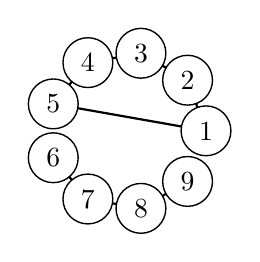
\begin{tikzpicture}
    \Vertices{circle}{1, 2, 3, 4, 5, 6, 7, 8, 9}
    \Edges(1, 2, 3, 4, 5, 1)
    \Edges(6, 7, 8, 9)
  \end{tikzpicture}
  \fi
\end{eg}

We need a bit more notations/definitions. Let \(G = (V, E)\) be a graph. If \(U \subseteq V\), the graph \(G - U\) is defined to be \(G - U = G[V \setminus U]\). If \(U = \{v\}\), write \(G - v = G - U\).

If \(F \subseteq E\), write \(G - F = (V, E \setminus F)\). If \(F = \{e\}\), write \(G - e = G - F\).

The \emph{complement}\index{complement} of \(G\) is the graph \(\overline G\) with
\begin{align*}
  V(\overline G) &= G \\
  E(\overline G) &= \{uv: u, v \in V, u \neq v, uv \neq E\}
\end{align*}

\begin{eg}\leavevmode
  \begin{enumerate}
  \item The complement of the complement graph \(K_n\) is the \emph{empty graph} of order \(n\), \(\overline K_n\), with \(n\) vertices and no edges.
  \item The complement of \(C_5\) is
    \begin{center}
    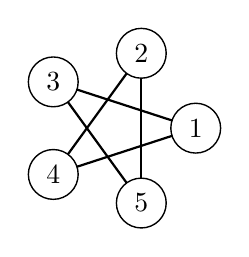
\begin{tikzpicture}
      \Vertices{circle}{1, 2, 3, 4, 5}
      \Edges(1, 3, 5, 2, 4, 1)
    \end{tikzpicture}
    \end{center}
    which is isomorphic to \(C_5\). We say \(C_5\) is \emph{self-complementary}.
  \end{enumerate}
\end{eg}

We say \(v, w \in G\) are \emph{adjacent}\index{adjacent} or \emph{neighbours} and write \(v \sim w\) if \(vw \in E\). The \emph{neighbourhodd} of \(v\) is
\[
  \Gamma(v) = \{w \in G: v \sim w\}.
\]
The \emph{degree}\index{degree} of \(v\) is the number of neighbours of \(v\): \(d(v) = |\Gamma(v)|\). More generally, if \(A \subseteq V\), the \emph{neighbourhood}\index{neighbourhood} of \(A\) is
\[
  \Gamma(A) = \bigcup_{v \in A} \Gamma(v).
\]
The \emph{minimum degree} of \(G\) is \(\delta(G) = \min_{v \in G} d(v)\). The \emph{maximum degree} of \(G\) is \(\Delta(G) = \max_{v \in G} d(v)\). The \emph{average degree} of \(G\) is
\[
  \overline d (G) = \frac{1}{|G|} \sum_{v \in G} d(v).
\]

Observe that
\begin{enumerate}
\item \(\delta(G) \leq \overline d(G) \leq \Delta(G)\). If either, i.e.\ both, are equalities we say \(G\) is \emph{regular}\index{graph!regular}. If \(G\) is regular, all vertices have the same degree. If that degree is \(r\), we say \(G\) is \emph{\(r\)-regular}.
\begin{eg}
  \(K_n\) is \((n - 1)\)-regular. \(\overline K_n\) is \(0\)-regular. \(C_n\) is \(2\)-regular. \(P_n\) is not regular for \(n \geq 2\) as \(\delta(P_n) = 1\) and \(\Delta(P_n) = 2\).
\end{eg}
\item \(2 e(G) = \sum_{v \in G} d(v)\). It is obvious as an edge has two ``ends''. A formal proof: let
  \[
    X = \{(e, v): e \in E, v \in e\}.
  \]
  To pick \((e, v) \in X\), we can choose \(e\) in \(e(G)\) ways then we choices for \(v\). So \(|X| = e(G) \times 2\). Alternatively, pick \(v\) first then, given \(v\), \(d(v)\) choices from \(e\) so \(|X| = \sum_{v\in G} d(v)\).

  This gives \(e(G) = \frac{|G| \overline d(G)}{2}\).
\end{enumerate}

A \emph{path}\index{path} in \(G\) from \(v\) to \(w\) where \(v, w \in G\), is a sequence \(v_0, v_1, \dots, v_\ell\) of distinct vertices of \(G\) where \(v_0 = v, v_\ell = w\) and \(v_{i - 1} \sim v_i\) for \(1 \leq i \leq \ell\). Usually write this path as \(v_0v_1\dots v_\ell\). The \emph{length}\index{length} of the path is \(\ell\). A path of length \(\ell\) in \(G\) yields a subgraph isomorphic to \(P_\ell\). In particular \(v\) is a path (of length \(0\)) from \(v\) to \(v\).

Define a relation \(\to\) on \(V(G)\) by \(v \to w\) if there is a path from \(v\) to \(w\). It is an equivalence relation (example sheet 2). The equivalence class of \(\to\) are the \emph{connected componenets}\index{connected componenets} of \(G\). Note \(G\) is the disjoint union of its components. If \(G\) has only one component, we say \(G\) is \emph{connected}\index{graph!connected}.

\begin{eg}
  A graph with three components (graph)
\end{eg}

A \emph{cycle of length \(n\)} in \(G\) is a subgraph of \(G\) isomorphic to \(C_n\). Often denote such by \(v_1v_2\dots v_nv_1\) where \(v_1, \dots v_n \in v(G)\) are distinct, \(v_{i - 1} \sim v_n\) for \(1 < i \leq n\) and \(v_n \sim v_1\). Note that unlike path, cycle does not have a starting point or direction. Thus there are many notations for some cycles, for example \(abcdea = dcbaed\).

A final notation: we often write \(e \in G\) to mean \(e \in E(G)\) if unambiguous.

\subsubsection{Bipartite graphs}

\begin{definition}[bipartite graph]\index{bipartite graph}
  A graph \(G = (V, E)\) is \emph{bipartite} if there is a partition \(V = X \cup Y\) such that any \(e \in E\) can be written \(e = xy\) where \(x \in X\), \(y \in Y\).

  The \emph{complete bipartite graph} \(K_{m, n}\) has \(|X| = m, |Y| = n\) and \(xy \in E(K_{m, n})\) for all \(x \in X, y \in Y\).
\end{definition}

\begin{eg}
  \(K_{2, 3}\)
  \iffalse
  \begin{center}
    \begin{tikzpicture}
      \Vertices{1, 2}
    \end{tikzpicture}
  \end{center}
  \fi
\end{eg}

In general, \(|K_{m, n}| = m + n, e(K_{m, n}) = mn\). There is a more useful characterisation of bipartite graphs:

\begin{proposition}
  A graph \(G = (V, E)\) is bipartite if and only if it contains no odd cycles.
\end{proposition}

\begin{proof}
  Suppose \(G = (V, E)\) is bipartite and \(V = X \cup Y\) is a partition. Assume for contradiction \(v_1v_2 \dots v_nv_1\) is a cycle with \(n\) odd. wlog \(v_1 \in X\). Then \(v_2 \in Y, v_2 \in X, \dots, v_n \in X, v_1 \in Y\). Contradiction.

  Suppose \(G\) has no odd cycles. wlog \(G\) is connected. Pick \(x \in G\). For \(y \in G\), define the distance from \(x\) to \(y\), \(d(x, y)\) to be the shortest path from \(x\) to \(y\). Let
  \[
    V_i = \{y \in G: d(x, y) = i\}
  \]
  for \(i \geq 0\). Let \(X = \bigcup_{i \text{ even}} V_i, Y = \bigcup_{i \text{ odd}} V_i\). Let \(uv \in E(G)\) with \(u \in V_j, v \in V_k\) where \(j \leq k\). Then must have \(k = j\) or \(k = j + 1\). Indeed there is a path of length \(j + 1\) from \(x\) to \(v\). 

  Suppose \(k = j\). We want to say that \(x, u\) and \(v\) form a cycle of length \(2j + 1\), but they may intersect somewhere earlier in the path. The standard way to deal with it is to take the closest intersection. Let \(u_0u_1 \dots u_j\) and \(v_0v_1 \dots v_j\) be shortest paths from \(x\) to \(u\) and \(v\) respectively, so \(u_0 = v_0 = x\), \(u_j = u\), \(v_j = v\) and \(u_i, v_i \in V_i\) for \(0 \leq i \leq j\). In particular, \(h \neq i\) implies that \(u_h \neq v_i\). Pick \(i\) largest such that \(u_i = v_i\), so \(0 \leq i < j\) and \(u_iu_{i + 1} \dots u_j v_j \dots v_i\) is a cycle of length \(2(j - i) + 1\) which is odd.
\end{proof}

\subsection{The forbidden subgraph problem}

\subsubsection{Complete subgraphs}

The problem of determining \(R(s)\) can be thought of as ``how many vertices can \(G\) have yet \(K_s \nsubseteq G\) and \(K_s \nsubseteq \overline G\)''. This is a typical example of an \emph{extremal problem}: how large can some parameter of a graph be before the graph is forced to have a certain property?

\begin{eg}
  Let \(|G| = n\). How large can \(e(G)\) get before \(G\) is forced to contain a triangle?

  The idea is to try \(G\) bipartite, as we know bipartite graphs do not contain triangles. Clearly we need complete bipartite graph so seek \(K_{s, t}\) where \(s + t = n\) so that \(E(K_{s, t}) = st = s(n - s)\) is maximised. This is achieved when \(s = \frac{n}{2}\) when \(n\) is even or \(s = \frac{n \pm 1}{2}\) when \(s\) is odd. Among bipartite graphs, \(K_{\floor{n/2}, \ceil{n/2}}\) is the best. Can we do better?

  Adding any edge to it creates a triangle but this isn't enough. For example, \(C_5\) is not bipartite but has the same property but clearly it isn't the best.
  \begin{center}
    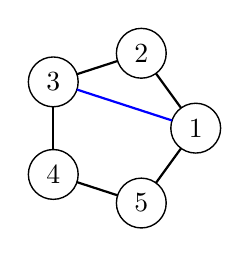
\begin{tikzpicture}
      \SetUpEdge[color = black]
      \Vertices{circle}{1, 2, 3, 4, 5}
      \Edges(1, 2, 3, 4, 5, 1)
      \SetUpEdge[color = blue]
      \Edges(1, 3)
    \end{tikzpicture}
  \end{center}
\end{eg}

In fact, bipartite always wins but we need to do some work.

\begin{proposition}[Mantel's theorem]\index{Mantel's theorem}
  Let \(|G| = n \geq 3, e(G) \geq \floor{\frac{n^2}{4}}\) and \(\triangle \nsubseteq G\). Then
  \[
    G \cong K_{\floor{n/2}, \ceil{n/2}}.
  \]
\end{proposition}

\begin{remark}
  It follows immediately that if \(|G| = n, e(G) > \floor{\frac{n^2}{4}}\) and \(\triangle \nsubseteq G\) then it is isomorphic to \(K_{\floor{n/2}, \ceil{n/2}}\) so \(e(G) = \floor{\frac{n^2}{4}}\), absurd. Thus \(K_{\floor{n/2}, \ceil{n/2}}\) has the most edges for a \(\triangle\)-free graph. The theorem asserts something stronger: it is \emph{uniquely} the best up to isomorphism.
\end{remark}

\begin{proof}
  Induction on \(n\). For \(n = 3\), \(|G| = 3, e(G) \geq 2, \triangle \nsubseteq G\) then \(G \cong K_{1, 2}\). For \(n \geq 4\), assume for now \(n\) is even so \(|G| = n, e(G) \geq \frac{n^2}{4}\), \(\triangle \nsubseteq G\). First delete edges from \(G\) if necessary to obtain a graph \(H\) with \(|H| = n, e(H) = \frac{n^2}{4}, \triangle \nsubseteq H\). Next pick \(v \in H\) of minimum degree and \(K = H - v\). Then \(|K| = n - 1\) and \(\triangle \nsubseteq K\). To bound \(e(K)\), note that
  \[
    d(v) = \delta(H) \leq \overline d(H) = \frac{1}{|H|} \sum_{x \in H} d(x)
    = \frac{1}{|H|} 2 e(H)
    = \frac{1}{n} \cdot 2 \frac{n^2}{4}
    = \frac{n}{2}
  \]
  so
  \[
    e(K) = e(H) - d(v)
    \geq \frac{n^2}{4} - \frac{n}{2}
    = \frac{(n - 1)^2}{4} - \frac{1}{4}
    = \floor*{\frac{(n - 1)^2}{4}}
  \]
  so by induction hypothesis
  \[
    K \cong K_{\floor{(n - 1)/2}, \ceil{(n - 1)/2}} = K_{\frac{n}{2} - 1, \frac{n}{2}}.
  \]
  To recover \(H\), we should add a vertex \(v\) to \(K\), joining it to precisely \(\frac{n}{2}\) vertices of \(K\) but creating no triangle. The only way to do this is to join \(v\) to all \(\ceil{\frac{n}{2}}\) vertices in one partition of \(K\). This thus gives \(H \cong K_{n/2, n/2}\).

  Finally \(G\) can be recovered by adding edges to \(H\) without making \(\triangle\). But this is impossible so \(G = H\), i.e.\ we did not in fact delete any edges in the beginning.

  \(n \geq 4\), \(n\) odd is similar.
\end{proof}

What about forbidding \(K_4\)? Should we try ``tripartite'' graphs?

\begin{definition}[\(r\)-partite]\index{graph!\(r\)-partite}
  A graph \(G\) is \emph{\(r\)-partite} if we can partition if \(V(G) = X_1 \cup X_2 \cup \dots \cup X_r\) such that \(u,v \in X_i\) for some \(i\) then \(u \nsim v\).

  It is \emph{complete \(r\)-partite} if \(u \in X_i, v \in X_j\) for \(i \neq j\) implies \(u \sim v\).
\end{definition}

Which \(r\)-bipartite graph of order \(n\) has most edges? Obviously such a \(G\) is complete \(r\)-bipartite. Suppose \(G\) has some two vertex classes \(X, Y\) with \(|X| \geq |Y| + 2\). Move a vertex \(v\) from \(X\) to \(Y\). We gain \(|X| - 1\) edges and lose \(|Y|\) edges. The net gain is \(|X| - 1 - |Y| \geq 1\), contradiction.

\begin{definition}[Turán graph]\index{Turán graph}
  The \emph{Turán graph} \(T_r(n)\) is the complete \(r\)-partite graph of order \(n\) with vertex classes as equal as possible. We write \(t_r(n) = e(T_r(n))\).
\end{definition}

\begin{eg}
  \(T_2(n) = K_{\floor{n/2}, \ceil{n/2}}\) and \(t_2(n) = \floor*{\frac{n^2}{4}}\). Mantel's theorem can be rephrased as to get most edges with no \(K_3\), take \(T_2(n)\).
\end{eg}

Some properties of Turán graphs:
\begin{enumerate}
\item \(K_{r + 1} \nsubseteq T_r(n)\) but adding any edge to \(T_r(n)\) makes a \(K_{r + 1}\).
\item If \(r \divides n\) then all vertex classes are the same size, namely \(\frac{n}{r}\). If \(r \ndivides n\), we have some small classes with \(\floor*{\frac{n}{r}}\) vertices and some large classes with \(\ceil*{\frac{n}{r}} = \floor*{\frac{n}{r}} + 1\) vertices.
\item Each vertex is joined to everyting except vertices in its own class. Therefore if \(r \divides n\) then \(T_r(n)\) is regular. If \(r \ndivides n\) then \(v \in T_r(n)\) in a large class has \(d(v) = \delta(T_r(n))\) whereas if \(v\) is in a small class, \(d(v) = \Delta(T_r(n)) = \delta(T_r(n)) + 1\). Hence in either case, give the order and average degree, the vertex degrees are as equal as possible.
\item What happens if we delete \(v \in T_r(n)\) of minimum degree? Then \(v\) is in a large class so we get \(T_r(n - 1)\). Therefore
  \[
    t_r(n) - \delta(T_r(n)) = t_r(n - 1).
  \]
\item Suppose we want to add a vertex \(v\) to \(T_r(n - 1)\) of as large degree as possible without making a \(K_{r + 1}\). We can't join \(v\) to a vertex in every class. So best is to join \(v\) to everything except a small class. This makes \(T_r(n)\). The biggest degree we can achieve for \(v\) is \(t_r(n) - t_r(n - 1)\) and only way to do this is to make \(T_r(n)\).
\end{enumerate}

\begin{theorem}[Turán]\index{Turán's theorem}
  Let \(|G| = n, e(G) \geq t_r(n)\) and \(K_{r + 1} \nsubseteq G\) (\(n \geq r + 1 \geq 3\)). Then \(G \cong T_r(n)\).
\end{theorem}

Note that Mantel's theorem is just a special case with \(r = 2\).

\begin{proof}
  Induction on \(n\). Suppose \(n = r + 1\). \(T_r(r + 1)\) has one class with two vertices and all other classes with one vertex, so \(T_r(r + 1)\) is \(K_{r + 1}\) minus an edge. For \(n > r + 1\), if necessary, delete edges from \(G\) to obtain \(H\) with \(|H| = n, e(H) = t_r(n)\) and \(K_{r + 1} \nsubseteq H\). Pick \(v \in H\) of minimum degree and let \(K = H - v\). Then \(|K| = n - 1\) and \(K_{r + 1} \nsubseteq K\). We know \(|H| = |T_r(n)|\) and \(e(H) = e(T_r(n))\) so
  \[
    \overline d(H) = \overline d(T_r(n)).
  \]
  But in \(T_r(n)\) vertex degrees are as equal as possible. Hence
  \[
    \delta(H) \leq \delta(T_r(n))
  \]
  and hence
  \[
    e(K) = e(H) - \delta(H) \geq t_r(n) - \delta(T_r(n)) = t_r(n - 1)
  \]
  so by induction hypothesis, \(K \cong T_r(n - 1)\). To recover \(H\) we need to add \(v\) to \(K\) of degree \(e(H) - e(K) = t_r(n) - t_r(n - 1)\) without making a \(K_{r + 1}\). So \(H \cong T_r(n)\). Adding an edge to \(H\) makes a \(K_{r + 1}\) so \(G = H \cong T_r(n)\).
\end{proof}

This is a special case of the \emph{forbidden subgraph problem}\index{forbidden subgraph problem}: fix a graph \(H\) with at least one edge. How many edges can a graph \(G\) of order \(n\) have yet not contain \(H\) as a subgraph?

Write
\[
  \exx(n; H) = \max \{e(G): |G| = n, H \nsubseteq G\},
\]
then Turán's theorem can be stated as \(\exx(n, K_{r + 1}) = t_r(n)\).

\subsubsection{Complete bipartite subgraphs}

What is \(\exx(n; C_4)\)? Suppose we have \(|G| = n, e(G) = m\) and \(C_4 \nsubseteq G\). How large can \(m\) be? The idea is to count the number of \(P_2\)-subgraphs, \(A\), in \(G\) in two different ways. Each \(v \in G\) is the middle vertex of \(\binom{d(v)}{2}\) \(P_2\)'s so
\[
  A = \sum_{v \in G} \binom{d(v)}{2}.
\]
Alternatively, as \(C_4 \nsubseteq G\), each pair of vertices are the end-vertices of at most one \(P_2\). (graph) so
\[
  A \leq \binom{n}{2}.
\]
It gives a bound on \(n\)
\[
  \binom{n}{2} \geq \sum_{v \in G} \binom{d(v)}{2}.
\]
The function \(x \mapsto \binom{x}{2}\) is convex so, writing \(\frac{m}{n} = a\),
\[
  \binom{n}{2} \geq \sum_{v \in G} \binom{d(v)}{2}
  \geq n \binom{\frac{1}{n} \sum_{v \in G} d(v)}{2}
  = n \binom{\frac{2m}{n}}{2}
  = n \binom{2a}{2}
\]
so
\[
  \frac{n(n - 1)}{2} \geq \frac{n 2a (2 a - 1)}{2}.
\]
Rearrange to get
\[
  4a^2 - 2a - (n - 1) \leq 0
\]
so
\[
  a \leq \frac{2 + \sqrt{4 + 16 (n - 1)}}{8} = \frac{1}{4}(1 + \sqrt{4n - 3})
\]
so
\[
  m \leq \frac{n}{4} (1 + \sqrt{4n - 3})
\]
and \(\exx(n; C_4) = O(n \sqrt n)\).

This is a fairly typical for extremal problesm --- usually we don't get exact answer but get some sort of bounds/aymptotics.

\begin{remark}\leavevmode
  \begin{enumerate}
  \item Note that we used \emph{Jensen's inequality}: let \(f: I \to \R\) be convex where \(I\) is an interval and \(x_1, \dots x_n \in I\). Then
    \[
      \frac{1}{n} \sum_{i = 1}^n f(x) \geq f(\frac{1}{n} \sum_{i = 1}^n x_i).
    \]
  \item Also a quick remark about binomial coefficients: if \(x \in \R\) and \(a \geq 0\) integer, we define
    \[
      \binom{x}{a} = \frac{x (x - 1) \dots (x - a + 1)}{a!}.
    \]
    Standard bounds:
    \[
      \binom{x}{a} \leq \frac{x^a}{a!}
    \]
    as long as \(x \geq a - 1\). On the other hand,
    \[
      \binom{x}{a} \geq \frac{(x - a + 1)^a}{a!} \geq \frac{1}{a!} \left(\frac{x}{2} \right)^a
    \]
    as long as \(x \geq 2 (a - 1)\). Usually when dealing with extremal graph problems, we suppose the parameters are sufficeintly large so these bounds apply.
  \item Note \(x \mapsto \binom{x}{2}\) is convex on \(\R\) but \(x \mapsto \binom{x}{a}\) is not. However, it is convex on \([a - 1, \infty)\), by writing \(y = x - a + 1\) to get a polynomial with positive coefficients.
  \end{enumerate}
\end{remark}

Let's go for \(\exx(n; K_{t, t})\) for \(t \geq 2\). We shall count \(t\)-fans (graph). In particular a \(2\)-fan is a \(P_2\) subgraph.

\begin{definition}[fan]\index{fan}
  A \emph{\(t\)-fan} in a graph \(G\) is an ordered pair \((v, U)\) where \(v \in G, U \subseteq V(G), |U| = t\) and for all \(u \in U, v \sim u\).
\end{definition}

\begin{theorem}
  \label{thm:forbidden complete bipartite subgraph}
  Let \(t \geq 2\). Then
  \[
    \exx(n; K_{t, t}) = O(n^{2 - \frac{1}{t}}).
  \]
\end{theorem}

\begin{proof}
  Let \(|G| = n, e(G) = m, K_{t, t} \nsubseteq G\). Let \(A\) be the number of \(t\)-fans in \(G\). To pick a \(t\)-fan \((v, U)\), can choose \(v \in G\) then \(U \subseteq \Gamma(v)\) with \(|U| = t\) so
  \[
    A = \sum_{v \in G} \binom{d(v)}{t}.
  \]
  As \(K_{t, t} \nsubseteq G\), for any \(U \subseteq V(G)\) with \(|U| = t\), there are at most \((t - 1)\) \(t\)-fans of the form \((v, U)\). So
  \[
    A \leq (t - 1) \binom{n}{t}.
  \]
  Technically we are done. To extract the explicit bound,
  \begin{align*}
    (t - 1) \frac{n^t}{t!}
    &\geq (t - 1) \binom{n}{t} \\
    &\geq A \\
    &= \sum_{v \in G} \binom{d(v)}{t} \\
    &\geq n \binom{\frac{1}{n} \sum_{v \in G} d(v)}{t} \\
    &= n \binom{\frac{2m}{n}}{t} \\
    &\geq \frac{n}{t!} \left(\frac{m}{n}\right)^t
  \end{align*}
  assuming \(\frac{m}{n}\) is sufficiently large. Hence
  \[
    \left( \frac{m}{n} \right)^t \leq (t - 1) n^{t - 1}
  \]
  and so
  \[
    m \leq (t - 1)^{\frac{1}{t}} n^{2 - \frac{1}{t}}.
  \]
\end{proof}

\begin{remark}\leavevmode
  \begin{enumerate}
  \item Why can we assume that \(\frac{m}{n}\) is sufficiently large? For lower bound on binomial coefficient, we need \(\frac{2m}{n} \geq 2(t - 1)\), i.e.\ \(m \geq (t - 1) n\). If not true then \(m < (t - 1)n\) so we don't care. Technically, we're really showing
    \[
      m < \max\{(t - 1)n , (t - 1)^{\frac{1}{t}} n^{2 - \frac{1}{t}} = O(n^{2 - \frac{1}{t}})\}.
    \]
  \item Can we use Jensen's inequality? We know \(x \mapsto \binom{x}{t}\) is convex on \([t - 1, \infty)\) and \(\binom{t - 1}{t} = 0\). Also we know if \(d(v) < t - 1\) then \(\binom{d(v)}{t} = 0\) so really we are apply Jensen's inequality to
    \[
      f(x) =
      \begin{cases}
        0 & x < t - 1 \\
        \binom{x}{t} & x \geq t - 1
      \end{cases}
    \]
    which is clearly convex. As \(\frac{m}{n}\) sufficiently large, \(\frac{2m}{n} \geq t - 1\) so \(f(\frac{2m}{n} = \binom{2m/n}{t}\).
\item This is closely related to the \emph{problem of Zarankiewicz}: we define
  \[
    Z(n, r) = \max \{e(G): \text{ \(G\) bipartite, \(n\) vertices in each class, \(K_{t, t} \nsubseteq G\)}\},
  \]
  the \emph{Zarankiewicz number}.
  \end{enumerate}
\end{remark}

\begin{corollary}
  Let \(t \geq 2\). Then
  \[
    Z(n, t) = O(n^{2 - \frac{1}{t}}).
  \]
\end{corollary}

\begin{proof}
  \[
    Z(n, t) \leq \exx(2n, K_{t, t}).
  \]
\end{proof}

\subsection{General subgraphs}

Let \(H\) be any graph with at least one dege. What is \(\exx(n; H)\)? It is too much to hope for exact results so we aim to find asymptotics. Consider, say,
\[
  \frac{\exx(n; H)}{\binom{n}{2}},
\]
``the proportion of edges of an \(H\)-free graph can have''. What happens as \(n \to \infty\)? If this converges, let
\[
  \exx(H) := \lim_{n \to \infty} \frac{\exx(n; H)}{\binom{n}{2}}.
\]

\begin{eg}\leavevmode
  \begin{enumerate}
  \item Turán: \(\exx(n, K_{r + 1}) = t_r(n) \approx (1 - \frac{1}{r}) \binom{n}{2}\). In fact \(\exx(K_{r + 1}) = 1 - \frac{1}{r}\).
  \item \(\exx(n, K_{t, t}) = O(n^{2 - \frac{1}{t}}) = o(n^2)\) so \(\exx(K_{t, t}) = 0\).
  \item For \(H\) any bipartite graph with at least one edge. Then \(H \subseteq K_{t, t}\) for some \(t\) so \(K_{t, t} \subseteq G\) implies that \(H \subseteq G\) so for all \(n\),
    \[
      \exx(n; H) \leq \exx(n; K_{t, t})
    \]
    so \(\exx(H) = 0\).
  \end{enumerate}
\end{eg}

\begin{proposition}
  Let \(H\) be a graph with at least one edge and let
  \[
    x_n = \frac{\exx(n; H)}{\binom{n}{2}}.
  \]
  Then \((x_n)\) converges.
\end{proposition}

\begin{proof}
  Let \(|G| = n\) and \(e(G) = \binom{n}{2} x_n\), \(H \nsubseteq G\). Suppose \(v \in G\). Then \(|G - v| = n - 1\) and \(H \nsubseteq G - v\) so
  \[
    e(G - v) \leq \binom{n - 1}{2} x_{n - 1}.
  \]
  Summing over \(v\) gives
  \begin{align*}
    & n \binom{n - 1}{2} x_{n - 1} \\
    \geq& \sum_{v \in G} e(G - v) = \sum_{v \in G} (e(G) - d(v)) \\
    =& n e(G) - 2e(G) = (n - 2) \binom{n}{2} x_n.
  \end{align*}
  Hence \(x_{n - 1} \geq x_n\). So \((x_n)\) is decreasing and bounded below by zero so converges.
\end{proof}

This shows that \(\exx(H) = \lim_{n \to \infty} \frac{\exx(n; H)}{\binom{n}{2}}\) exists. Can we find it? This is answered in full by the following theorem

\begin{notation}
  \(K_r(t)\) is the complete \(r\)-bipartite graph with \(t\) vertices in each class. This is the same as the Turán graph \(T_r(rt)\).
\end{notation}

\begin{theorem}[Erdős-Stone]\index{Erdős-Stone theorem}
  \label{thm:Erdős-Stone theorem}
  Let \(r, t \geq 1\) be integers and \(\varepsilon > 0\) be real. Then there exists an integer \(n_0\) such that for all \(n \geq n_0\), if \(|G| = n, e(G) \geq (1 - \frac{1}{r} + \varepsilon) \binom{n}{2}\) then \(K_{r + 1}(t) \subseteq G\).
\end{theorem}

Before we give the proof, we have to ask what this not so obvious statement means. Using notation in the statement of the theorem, Turán says that if density of edges is around \(1 - \frac{1}{r}\) then \(K_{r + 1} \subseteq G\). What happens if we make a tiny increase in the density? Erdős-Stone tells us that we get much, much more --- we get enormous ``blown-up'' \(K_{r + 1}\)'s as well. Of course this is provided \(G\) has sufficiently many vertices.

We will get to the proof later but we can prove the case \(r = 1\). It says that for \(|G| = n, e(G) \geq \varepsilon \binom{n}{2}\) then \(K_{t, t} \subseteq G\) for \(n\) sufficiently large. But this follows from \Cref{thm:forbidden complete bipartite subgraph}:
\[
  \exx(n; K_{t, t}) = O(n^{2 - \frac{1}{t}}) = o(n^2).
\]

\begin{definition}[chromatic number]\index{chromatic number}
  The \emph{chromatic number} of a graph \(H\) is the least \(r\) such that \(H\) is \(r\)-partite. It is denoted \(\chi(H)\).
\end{definition}

\begin{corollary}
  \label{cor:forbidden subgraph and chromatic number}
  Let \(H\) be a graph with at least one edge. Then
  \[
    \exx(H) = 1 - \frac{1}{\chi(H) - 1}.
  \]
\end{corollary}

\begin{proof}
  Let \(\chi(H) = r + 1\) and choose \(t\) such that \(H \subseteq K_{r + 1}(t)\) (e.g.\ \(t = |H|\)). Let \(\varepsilon > 0\). By Erdős-Stone there is some \(n_0\) such that if \(|G| = n \geq n_0\) and \(e(G) \geq (1 - \frac{1}{r} + \varepsilon) \binom{n}{2}\) then \(K_{r + 1}(t) \subseteq G\). But then also \(H \subseteq G\). So this says that if \(n \geq n_0\) then
  \[
    \exx(n; H) \leq (1 - \frac{1}{r} + \varepsilon) \binom{n}{2}
  \]
  and so
  \[
    \frac{\exx(n; H)}{\binom{n}{2}} \leq 1 - \frac{1}{r} + \varepsilon.
  \]
  Take limit as \(n \to \infty\), get
  \[
    \exx(H) \leq 1 - \frac{1}{r} + \varepsilon.
  \]
  As \(\varepsilon\) is arbitrary,
  \[
    \exx(H) \leq 1 - \frac{1}{r} = 1 - \frac{1}{\chi(H) - 1}.
  \]

  On the other hand, for all \(n\), \(H \nsubseteq T_r(n)\). This means that for all \(n\), \(\exx(n; H) \geq t_r(n)\) so
  \[
    \frac{\exx(n; H)}{\frac{n}{2}} \geq \frac{t_r(n)}{\binom{n}{2}} \to 1 - \frac{1}{r}
  \]
  as \(n \to \infty\). So we get the other inequality. The result follows.
\end{proof}

We have now solved the forbidden subgraph problem aymptotically for non-bipartite \(H\). Then \Cref{cor:forbidden subgraph and chromatic number} implies that
\[
  \exx(n; H) \sim (1 - \frac{1}{\chi(H) - 1}) \binom{n}{2}.
\]
The situation is not so good if \(H\) is bipartite, in which case \Cref{cor:forbidden subgraph and chromatic number} says that \(\exx(H) = 0\), i.e.\ \(\exx(n, H)\) grows slower than \(\binom{n}{2}\) but does not give the asymptotic rate of growth.

\begin{eg}\leavevmode
  \begin{enumerate}
  \item For \(t = 2\), \(\exx(n, K_{t, t}) = O(n^{2 - \frac{1}{t}})\) so \(\exx(n; K_{2, 2}) = O(n^{\frac{3}{2}})\). In fact \(\exx(n; K_{2, 2}) = \Theta(n^{3/2})\).
  \item For \(t = 3\), \(\exx(n; K_{3, 3}) = O(n^{5/3})\). In fact, \(\exx(n; K_{3, 3}) = \Omega(n^{5/3})\).
  \item For \(t = 4\), \(\exx(n; K_{4, 4}) = O(n^{7/4})\). At this moment, no one knows if \(\exx(n; K_{4, 4}) = \Omega(n^{7/4})\).
  \end{enumerate}
\end{eg}

\begin{notation}
  Big-\(O\) notation and its cousins:
\begin{align*}
  f &= O(g) \text{ if } f< Ag \text{ for some constant } A \\
  f &= \Omega(g) \text{ if } g=O(f) \\
  f &= \Theta(g) \text{ if } f= O(g) \text{ and } f = \Omega(g).
\end{align*}
Also,
\begin{align*}
  f &= o(g) \text{ if } f/g\to 0 \text{ as } n\to \infty \\
  f &= \omega(g) \text{ if } f/g\to \infty \\
  f &\sim g \text{ if } f/g\to 1.
\end{align*}
\end{notation}

It's been conjectured that
\[
  \exx(n, K_{t, t}) = \Omega(n^{2 - \frac{1}{t}})
\]
for all \(t \geq 2\) but the problem remains unproven for \(n > 3\). Therefore even asymptotically, forbidden subgraph problem has not been solved for bipartite \(H\).

As another application of Erdős-Stone, we define

\begin{definition}[density]\index{density}
  Let \(G\) be a graph. The \emph{density} of \(G\) is
  \[
    D(G) = \frac{e(G)}{\binom{|G|}{2}}.
  \]
\end{definition}

\begin{definition}[upper density]\index{upper density}
  Let \(G\) now be an infinite graph. The \emph{upper density} of \(G\) is the limit of the maximum densities of finite subgraphs, i.e.\
  \[
    \ud(G) = \lim_{n \to \infty} \sup \{D(H): H \subseteq G, |H| = n\}.
  \]
\end{definition}

See example sheet 2 for its existence, or if you're patient, we will prove it in a moment.

We have \(\ud(G) \in [0, 1]\). A priori, \(\ud(G)\) may take any value in \([0, 1]\) but in fact

\begin{corollary}
  Let \(G\) be an infinite graph. Then
  \[
    \ud(G) \in \{1\} \cup \{1 - \frac{1}{r}: r = 1, 2, \dots\}.
  \]
\end{corollary}

\begin{proof}
  Let
  \[
    x_n = \sup \{D(H): H \subseteq G: |H| = n\}.
  \]
  Enough to show that if
  \[
    \limsup_{n \to \infty} x_n > 1 - \frac{1}{r}
  \]
  then
  \[
    \liminf_{n \to \infty} x_n \geq 1 - \frac{1}{r + 1}.
  \]
  Suppose \(\limsup_{n \to \infty} x_n > 1 - \frac{1}{r}\). Pick \(\varepsilon > 0\) such that
  \[
    1 - \frac{1}{r} + \varepsilon < \limsup_{n \to \infty} x_n,
  \]
  meaning that we can find a sequence \((H_j)\) of subgraphs of \(G\) with \(|H_j| = n_j \to \infty\) and \(D(H_j) \geq 1 - \frac{1}{r} + \varepsilon\). By Erdős-Stone, for any \(t\), if \(j\) is sufficiently large then \(K_{r + 1}(t) \subseteq H_j \subseteq G\). Then for any \(n\), if \(t\) is suffciently large we have \(T_{r + 1}(n) \subseteq K_{r + 1}(t) \subseteq G\). Then
  \[
    x_n \geq D(T_{r + 1}(n)) = \frac{t_{r + 1}(n)}{\binom{n}{2}} \to 1 - \frac{1}{r + 1}
  \]
  so
  \[
    \liminf_{n \to \infty} x_n \geq 1 - \frac{1}{r + 1}.
  \]
\end{proof}

\begin{proof}[Proof of \nameref{thm:Erdős-Stone theorem}]
  Sketch of proof, nonexaminable. The proof bears much similarity with that of \(\exx(n;, K_{t, t}) = O(n^{2 - \frac{1}{t}}\). In the statement of the theorem there is a condition on \(e(G)\). This is a global condition and does not give any restriction on a vertex, which we used to obtain an inequality on the number of \(t\)-fans previously. We want to convert it into a local condition, i.e.\ we'd rather prefer a lower bound on \(\delta(G)\). We begin with a technical lemma.
  \begin{lemma}
    Let \(\alpha, \varepsilon > 0\). Then there exists \(\gamma > 0\) and an integer \(n_0\) such that if \(|G| = n \geq n_0\) and \(e(G) \geq (\alpha + \varepsilon) \binom{n}{2}\) then there is \(H \subseteq G\) with \(|H| = n' \geq \gamma n\) and \(\delta(H) \geq \alpha n'\).
  \end{lemma}

  \begin{proof}[Sketch of proof]
    Keep deleting vertices of minimum degree and do an unpleasant calculation.
  \end{proof}

  So we can reformulate the theorem as:

\begin{theorem}
  Let \(r, t \geq 1\) be integers and \(\varepsilon > 0\). Then there is some \(n_0\) such that for all \(n \geq n_0\),
  \[
    |G| = n, \delta(G) \geq (1 - \frac{1}{r} + \varepsilon) n
  \]
  then
  \[
    K_{r + 1}(t) \subseteq G.
  \]
\end{theorem}

\begin{proof}
  Induction on \(r\). If \(r = 1\) then let \(|G| = n, \delta(G) \geq \varepsilon n\). So
  \[
    e(G) \geq \frac{n\delta(G)}{2} = \frac{\varepsilon n^2}{2}.
  \]
  But
  \[
    \exx(n; K_2(t)) = O(n^{2 - \frac{1}{n}})
  \]
  so for \(n\) sufficiently large,
  \[
    \exx(n; K_2(t)) < \frac{\varepsilon n^2}{2}
  \]
  and so \(K_2(t) \subseteq G\).

  For \(r > 1\), suppose the result is false for some \(r \geq 2, t \geq 1, \varepsilon > 0\). Fix \(T\) ``large''. Pick \(n_0\) such that if \(n \geq n_0\) then \(|G| = n\) and
  \[
    \delta(G) \geq (1 - \frac{1}{r} + \varepsilon)n
  \]
  then \(K_r(T) \subseteq G\), which exists by induction hypothesis since \(1 - \frac{1}{r} > 1 - \frac{1}{r - 1}\). We can find a graph \(G\) with \(|G| = n  \geq n_0\), \(\delta(G) \geq (1 - \frac{1}{r} + \varepsilon)n\) but \(K_{r + 1}(t) \nsubseteq G\). Note that we can choose \(n\) to be as large as we like. We know \(K_r(T) \subseteq G\). Let \(V_1, \dots, V_r\) be the vertex sets of a \(K_r(T) \subseteq G\).

  We now use the fan-counting trick (graph). Let
  \[
    X = \{(v_1, \dots, v_r, U): v_i \in V_i \text{ for all } 1 \leq i \leq r, u \sim v_i \text{ for all } u \in U\}
  \]
  be the ``generalised fans''. To pick \((v_1, \dots, v_r, U) \in X\) we could pick the \(v_i\)'s first (\(T\) choices each) then pick \(U \subseteq \bigcap_{i = 1}^r \Gamma(v_i)\) with \(|U| = t\). Now
  \begin{align*}
    &\big| \bigcap_{i = 1}^n \Gamma(v_i) \big| = |G| - \big| \bigcup_{i = 1}^r G \setminus \Gamma(v_i) \big| \geq |G| - \sum_{i = 1}^r |G \setminus \Gamma(v_i)| \\
    =& n - \sum_{i = 1}^r (n - |\Gamma(v_i)|) \geq n - r (\frac{1}{r} - \varepsilon) n = r \varepsilon n
  \end{align*}
  so
  \[
    |X| \geq T^r \binom{r \varepsilon n}{t}.
  \]
  Suppose instead we pick \(U\) first. As \(K_{r + 1}(t) \nsubseteq G\), there cannot be \(t\) possible choices for each \(v_i\) so
  \[
    |X| \leq \binom{n}{t} (t - 1) T^{r - 1}.
  \]
  Note that we're basically done here since it can't be the case that \(T^{r - 1} \lesssim |X| \lesssim T^r\) as \(T\) is arbitrary. Concretely,
  \begin{align*}
    &\frac{n^t}{t!} (t - 1) T^{r - 1}
      \geq \binom{n}{t} (t - 1) T^{r - 1}
      \geq |X| \\
    & \geq T^r \binom{r\varepsilon n}{t}
      \geq T^r (\frac{r \varepsilon n}{2})^t \frac{1}{t!}
  \end{align*}
  for \(n\) sufficiently large so
  \[
    t - 1 \geq T (\frac{r\varepsilon}{2})^t
  \]
  so
  \[
    T \leq (t - 1) (\frac{2}{r \varepsilon})^t.
  \]
  But \(T\) is arbitrary, absurd.
\end{proof}
\end{proof}

\subsection{Hamilton cycles}

\begin{definition}[Hamilton cycle]\index{Hamiltonian cycle}\index{graph!Hamiltonian}
  A \emph{Hamilton cycle} in a graph \(G\) is a cycle in \(G\) of length \(|G|\).

  We say \(G\) is \emph{Hamiltonian} if it contains such a cycle.
\end{definition}

We can ask extremal questions for Hamiltonian cycles. If \(|G| = n\) for some fixed \(n\), how large can \(e(G)\) be without \(G\) being Hamiltonian? The answer is not very interesting --- we can have \(G\) non-Hamiltonian with almost all edges present by removing \(n - 2\) edges from a vertex in \(K_n\). As better question is to ask upper bound in \(\delta(G)\).

\begin{theorem}[Dirac]\index{Dirac's theorem}
  Let \(|G| \geq 3\) and \(\delta(G) \geq \frac{n}{2}\). Then \(G\) is Hamiltonian.
\end{theorem}

\begin{proof}
  First, \(G\) is connected: indeed, suppose \(x, y \in G\) with \(x \nsim y\). We have
  \[
    |\Gamma(x) \cup \Gamma(y)| \leq n - 2
  \]
  but
  \[
    |\Gamma(x)| + |\Gamma(y)| \geq \frac{n}{2} + \frac{n}{2} = n > n - 2
  \]
  so exists \(z \in \Gamma(x) \cap \Gamma(y)\).

  Let \(v_0 v_1 \dots v_\ell\) be a path in \(G\) of maximal length. By maximality,
  \begin{align*}
    \Gamma(v_0) &= \{v_1, \dots, v_\ell\} \\
    \Gamma(v_\ell) &= \{v_0, \dots, v_{\ell - 1}\}
  \end{align*}
  To show it is part of a cycle, we want to show it ``doubles back'' at both endpoints. Let
  \begin{align*}
    A &= \{i \in [\ell]: v_0 \sim v_i\} \\
    B &= \{i \in [\ell]: v_\ell \sim v_{i - 1}\}
  \end{align*}
  Then
  \[
    |A| + |B| \geq \frac{n}{2} + \frac{n}{2} = n
  \]
  but
  \[
    |A \cup B| \leq \ell \leq n - 1 < |A| + |B|
  \]
  so exists \(i \in A \cap B\) and \(C = v_0v_i \dots v_\ell v_{i - 1} v_{i - 2} \dots v_0\) is a cycle of length \(\ell + 1\) in \(G\). If \(\ell + 1 = n\) then \(G\) is Hamiltonian. If not, relabel \(C = v_0 v_1 \dots v_\ell v_0\). As \(G\) is connected there is some \(v_j \in C\) and some \(w \in G - C\) with \(w \sim v_j\). Then \(w v_j v_{j + 1} \dots v_\ell v_0 \dots v_{j - 1}\) is a path in \(G\) of length \(\ell + 1\), contradicting maximality.
\end{proof}

This is the best possible result. For \(|G| = n\) even, \(K_{n/2} \cup K_{n/2}\) has \(\delta(G) = \frac{n}{2} - 1\) but dissconnected. For \(|G| = n\) odd, let \(G\) be two copies of \(K_{(n + 1)/2}\) with one edge between them.

We can prove more by same method.

\begin{proposition}
  Let \(G\) be connected and \(|G| = n, \delta(G) \geq k\) where \(2 \leq k < \frac{n}{2}\). Then \(G\) must contain a path of length \(2k\) and a cycle of length at least \(k + 1\).
\end{proposition}

\begin{proof}
  Take \(v_0v_1 \dots v_\ell\) and \(A, B\) as in the previous proof. Suppose \(\ell < 2k\) then
  \[
    |A| + |B| \geq k + k = 2k > \ell \geq |A \cup B|
  \]
  so as before we can find a longer path, contradiction. So \(G\) has a path of length \(2k\).

  Let \(i = \max A\). Then \(v_0v_1 \dots v_iv_0\) is a cycle of length \(i + 1\). But \(i \geq |A| \geq k\).
\end{proof}

\begin{remark}
  We can't guarantee a cycle of length exactly \(k + 1\). For example, take \(n = 5, k = 2\) and \(G = C_5\).
\end{remark}

\subsubsection{Eulerian graphs}

\begin{definition}[circuit, Eulerian]\index{circuit}\index{graph!Eulerian}
  A \emph{circuit} in a graph \(G\) (of length \(\ell\)) is a sequence \(v_0v_1 \dots v_\ell\) of not-necessarily distinct vertices of \(G\) such that \(v_0 = v_\ell\) and if \(1 \leq i \leq \ell\) then \(v_{i - 1}v_i \in E(G)\) and if \(1 \leq i < j \leq \ell\) then \(v_{i - 1} v_i \neq v_{j - 1} v_j\).

  If for all \(e \in E(G)\) we have \(e = v_{i - 1}v_i\) for some \(i\) we say the circuit is an \emph{Euler circuit}. If \(G\) has an Euler circuit, we say \(G\) is \emph{Eulerian}.
\end{definition}

\begin{proposition}
  Let \(G\) be connected. Then \(G\) is Eulerian if and only if every vertex has even degree.
\end{proposition}

\begin{proof}
  In an Euler circuit, each vertex appears the same number of times as a ``first'' vertex and as a ``second'' vertex of an edge.

  Conversely, if every vertex has even degree then we start from a circuit and keep augementing it until we've travelled along each edge. Formally, induction on \(e(G)\). If \(e(G) = 0\) then done. If \(e(G) > 0\), let \(v_0v_1\dots v_\ell\) be a longest possible circuit. Easy to check it is non-trivial, i.e.\ \(\ell > 0\). Write \(C = v_0 v_1 \dots v_\ell\). If \(C\) is Euler circuit then done. Otherwise let
  \[
    F = \{v_{i - 1}v_i: 1 \leq i \leq \ell\} \subseteq E(G).
  \]
  Then \(e(G - F) > 0\) and each vertex of \(G - F\) has even degree. Moreover, \(C\) meets every component of \(G - F\). Let \(H\) be a component of \(G - F\) with at least one edge. By induction hypothesis, \(H\) has Euler circuit \(D = w_0w_1 \dots w_m\), say. \(C\) and \(D\) must meet, wlog \(v_0 = w_0\). Then \(v_0v_1 \dots v_{\ell - 1} w_0w_1 \dots w_n\) is a longer circuit in \(G\) than \(C\), contradiction.
\end{proof}

By running the proof on a multigraph we can show that Königsberg problem has a negative answer.

\section{Graph colouring}

\subsection{Planar graphs}

Let's return to the map-colouring problem from chapter 0.

\begin{definition}[colouring]\index{colouring}
  A \emph{\(k\)-colouring} of a graph \(G\) is a function \(c: V(G) \to [k]\) such that if \(uv \in E(G)\) then \(c(u) \neq c(v)\).
\end{definition}

\begin{note}
  Unfortunately the definition is in conflict with colouring in Ramsey theory sense. However, context should always be clear which one we're referring to.
\end{note}

As we defined graph as an abstract structure built on a set, although it is obvious what we mean by a ``drawing'' and we frequently employ such graphical representations in practice, we still have to make a formal definition. It is slightly irritating and you can forget about it as soon as we have defined it.

\begin{definition}[drawing]
  A \emph{(plane) drawing} of a graph \(G = (V, E)\) is an ordered pair \((\varphi, \Gamma)\) where \(\varphi: V \to \R^2\) is an injection and \(\Gamma = \{\gamma_e: e \in E\}\) where for each \(e \in E\), \(\gamma_e: [0, 1] \to \R^2\) is a continuous injection satisfying
  \begin{enumerate}
  \item for all \(uv \in E\), \(\{\gamma_{uv}(0), \gamma_{uv}(1)\} = \{\varphi(u), \varphi(v)\}\);
  \item if \(e, f \in E\) with \(e \neq f\) then \(\gamma_e((0, 1)) \cap \gamma_f((0, 1)) = \emptyset\),
  \item for all \(e \in E, v \in V\), \(\varphi(v) \notin \gamma_e((0, 1))\).
  \end{enumerate}
\end{definition}

\begin{definition}[planar graph]\index{graph!planar}
  If \(G\) has a drawing we say \(G\) is \emph{planar}.
\end{definition}

\begin{remark}
  As we defined drawing as topological objects, it is reasonable to worry about pathological drawings of a graph, for example, if one of the path is a space-filling curve. However, it turns out that if \(G\) has a drawing, then it has a drawing in which the image of each \(\gamma_e\) is a finite union of line segments. Henceforth assume all drawings like this. However it is more convenient to draw an arc between vertices to represent a finite sequence of ``zig-zag'' line segments.
\end{remark}

The natural question is: how many colours do we need to colour a planar graph? Before we attempt to answer the question, we should try to understand planar graphs.

\begin{eg}\leavevmode
  \begin{enumerate}
  \item \(K_3\) is planar. (graph)
  \item \(K_4\) is planar. (graph)
  \item What about \(K_5\)? Let \(\{v, w, x, y, z\} = V(G)\). \(K_5\) has a \(5\)-cycle \(vwxyz\), which in a draing separates \(\R^2\) into ``inside'' and ``outside'' (we don't need Jordan curve drawing since we have line segments). Need to add \(vx, wy, xz, yv, zw\). wlog \(vx\) is inside and \(wy\) is outside. Then \(xz\) has to be inside, \(yv\) outside. Now can't draw \(zw\) so \(K_5\) is not planar.
  \item A similar argument shows \(K_{3, 3}\) is not planar: let \(\{a, b, c\}\) and \(\{x, y, z\}\) be the vertex classes. Have a \(6\)-cycle \(axbycza\). Need to add \(ay, bz, cx\). At most one can be drawn outside and at most one inside, so \(K_{3, 3}\) not planar.
  \end{enumerate}
\end{eg}

Are there any other graph other than \(K_5, K_{3, 3}\) that is nonplanar? Obviously if \(K_5 \subseteq G\) or \(K_{3, 3} \subseteq G\) then \(G\) is nonplanar. It seems that there should be more ``classes'' of nonplanar graphs but surprisingly, this is essentially the only obstacle to planarity. Here essentially means the inclusion of ``stupid'' examples such as replace an edge into a path with more than two vertices in \(K_{5, 5}\). This is not planar as otherwise we can contract some of the edges and obtain a drawing ob \(K_{5, 5}\).

\begin{definition}[subdivision]\index{subdivision}
  A graph \(H\) is a \emph{subdivision} of a graph \(G\) if \(H\) can be formed from \(G\) by repeated doing: pick \(uv \in E(G)\), delete \(uv\), add new vertex \(w\) and edge \(uw, vw\).
\end{definition}

\begin{theorem}[Kuratowski]\index{Kuratowsi's theorem}
  \(G\) is planar if and only if \(G\) has a subdivision of neither \(K_5\) or \(K_{3, 3}\) as a subgraph.
\end{theorem}

\begin{proof}
  Non-examinable. Omitted.
\end{proof}

\begin{definition}[forest/acyclic graph, tree, leaf]\index{forest}\index{graph!acyclic}\index{tree}\index{leaf}
  A \emph{forest} is a graph with no cycles. It is also called an \emph{acyclic} graph.

  A \emph{tree} is a connected forest.

  A \emph{leaf} is a vertex of degree \(1\).
\end{definition}

\begin{remark}\leavevmode
  \begin{enumerate}
  \item A forest is a disjoint union of trees.
  \item Every connected graph  \(G\) has a \emph{spanning tree}\index{spanning tree} \(T\), i.e.\ a subgraph \(T\) with \(V(T) = V(G)\) and \(T\) a tree, by removing edges from cycles until it is acyclic.
  \end{enumerate}
\end{remark}

\begin{proposition}
  Every nontrivial tree has a leaf.
\end{proposition}

\begin{proof}
  Let \(T\) be a tree and \(v_0v_1 \dots v_\ell\) be a maximal-length path in \(T\). Then \(v_\ell\) has no neighbour in the path except \(v_{\ell - 1}\) (as \(T\) is acyclic) and no neighbours outside the path (by maximality) so \(v_\ell\) is a leaf.
\end{proof}

This is a not so surprising result that is not difficult at all either. However it comes in handy when we want to convert our intuition for a tree into a formal proof about its property (hint: induction!).

\begin{proposition}
  \label{prop:edge of tree}
  Let \(T\) be a tree with \(|T| = n \geq 1\). Then \(e(T) = n - 1\).
\end{proposition}

\begin{proof}
  Induction on \(n\). Holds for \(n = 1\). For \(n >1\), let \(v\) be a leaf of \(T\). Then \(T - v\) is a tree with order \(n - 1\). By induction hypothesis \(e(T - v) = n - 2\) so \(e(T) = n - 1\).
\end{proof}

\begin{proposition}
  Every forest is planar.
\end{proposition}

\begin{proof}
  Enough to show that every tree \(T\) is planar. Induction on \(n = |T|\). Holds for \(n = 1\). For \(n > 1\), let \(v \in T\) be a leaf and \(u\) the neighbour of \(v\). By induction hypothesis, \(T - v\) has a drawing. On a sufficiently small ball around \(u\) in \(\R^2\), there are finitely many radial segments. So can add \(v\) and \(uv\) to the drawing.
\end{proof}

Any drawing of a planar graph divides the plane divides the plane into connected regions, called \emph{faces}\index{face}. Precisely one is unbounded, called the \emph{infinite face}.

\begin{center}
  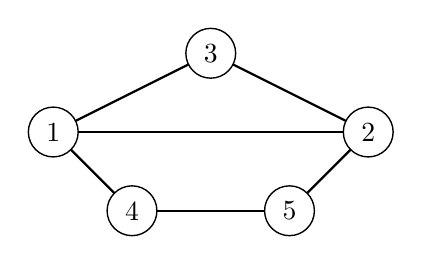
\begin{tikzpicture}
    \Vertex[x=0,y=0]{1}
    \Vertex[x=4,y=0]{2}
    \Vertex[x=2,y=1]{3}
    \Vertex[x=1,y=-1]{4}
    \Vertex[x=3,y=-1]{5}
    \Edges(1, 2, 3, 1)
    \Edges(1, 4, 5, 2)
  \end{tikzpicture}
\end{center}
which has 3 faces. The infinite face has 5 edges.

We can also draw it differently
\begin{center}
  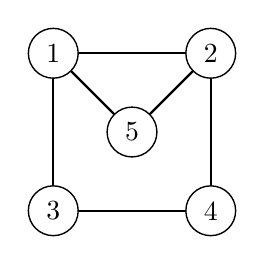
\begin{tikzpicture}
    \Vertex[x=0,y=0]{1}
    \Vertex[x=2,y=0]{2}
    \Vertex[x=0,y=-2]{3}
    \Vertex[x=2,y=-2]{4}
    \Vertex[x=1,y=-1]{5}
    \Edges(1, 2, 4, 3, 1, 5, 2)
  \end{tikzpicture}
\end{center}

in which case the infinite face has 4 edges. Even worse, we can produce drawing with \(3, 3, 4, 6\) edges and \(3, 3, 5, 5\) edges (graph). Thus face is an object associated with a drawing, not with a graph. However, there does exists a drawing invariant of a graph: the number of faces.

\begin{theorem}[Euler's formula]\index{Euler's formula}
  Let \(G\) be a connected planar graph, \(|G| = n \geq 1, e(G) = m\). Suppose \(G\) can be drawn with \(\ell\) faces. Then
  \[
    n - m + \ell = 2.
  \]
\end{theorem}

Thus sometimes we can make statements like ``a certain graph has 17 faces''.

\begin{proof}
  Induction on \(m\). If \(G\) is a tree then clearly \(\ell = 1\) and by \Cref{prop:edge of tree}, \(m = n - 1\) so
  \[
    n - (n - 1) + 1 = 2.
  \]
  For general \(G\), take a drawing of \(G\) and pick an edge \(e\) in a cycle in \(G\). Delete \(e\) from \(G\) and the drawing. Now have a drawing of \(G - e\) with \(\ell - 1\) faces. Also \(G - e\) is connected with \(|G - e| = n, e(G - e) = m - 1\). By induction hypothesis,
  \[
    n - (m - 1) + (\ell - 1) = 2
  \]
  so
  \[
    n - m + \ell = 2.
  \]
\end{proof}

Using Euler's formula, we can get a much better bound on the number of vertices a planar graph than \(\binom{n}{2}\).

\begin{theorem}
  Let \(G\) be planar with \(|G| = n \geq 3\). Then
  \[
    e(G) \leq 3n - 6.
  \]
\end{theorem}

\begin{proof}
  There is one special case which we single out first. If \(G \cong P_2\) then the result holds so suppose it isn't. Given a drawing of \(G\) with \(\ell\) faces, wlog \(G\) is connected (add edges if necessary), by Euler's formula we know \(n - m + \ell = 2\). Each edge borders at most 2 faces and each face is bordered by at least 3 edges so
  \[
    \ell \leq \frac{2}{3} m
  \]
  so
  \[
    2 \leq n - m + \frac{2}{3} m.
  \]
  Rearrange to get the desired result.
\end{proof}

\begin{proposition}[six-colour theorem]
  Every planar graph is 6-colourable.
\end{proposition}

\begin{proof}
  Let \(G\) be planar with \(|G| = n\). Induction on \(n\). For \(n \leq 6\) this is obviously true. For \(n > 6\), pick \(v \in G\) of minimal degree. By induction hypothesis we can 6-colour \(G - v\). But
  \[
    d(v) = \delta(G) \leq \frac{2 e(G)}{n} \leq \frac{6n - 12}{n} < 6
  \]
  so \(d(v) \leq 5\). So some colour is missing on \(\Gamma(v)\). Use this to colour \(v\).
\end{proof}

That feel like a enourmous progress to bring down the number from infinity to 6. With some more work, we can do better.

\begin{theorem}[five-colour theorem]
  Every planar graph is 5-colourable.
\end{theorem}

\begin{proof}
  Let \(G\) be planar with \(|G| = n\). Induction on \(n\). Obvious for \(n \leq 5\). For \(n > 5\), as in the proof of 6-colour theorem, pick \(v \in G\) with \(d(v) \leq 5\) and by induction hypothesis there exists a 5-colouring of \(G - v\). If some colour is missing from \(\Gamma(v)\) then done. Otherwise consider a drawing of \(G\) in which \(v\) has neighbours \(x_1, \dots, x_5\) in clockwise order around \(v\) with \(c(x_i) = i\) wlog. The strategy is to change colouring of \(x_1\) from \(1\) to \(3\), and ``propagate the change'' retrogradely until all things are done. There is one case it might not work, namely there is a \(13\)-path between \(x_1\) and \(x_3\), as in the end we just swapped the colouring on the two vertices.

  Formally, suppose that there is no 13-path from \(x_1\) to \(x_3\), i.e.\ a path all of whose vertices have colour 1 or 3. Then swap colours 1 and 3 on the 13-component of \(x_1\), i.e.\ the component containing \(x_1\) of the subgraph \(G[W]\) where \(W = \{x \in G: c(x) = 1 \text{ or } 3\}\). Now can give \(v\) colour \(1\).

  Suppose instead there is such a 13-path. Then there is no 24-path from \(x_2\) to \(x_4\) so swap colours 2, 4 on 24-component of \(x_2\). Then give \(v\) colour 2.
\end{proof}

Can we still do better? In fact we can.

\begin{theorem}[four-colour theorem]
  Every planar graph is 4-colourable.
\end{theorem}

\begin{proof}[False proof, non-examinable]
  Let \(G\) be planar with \(|G| = n\). Induction on \(n\). Obvious for \(n \leq 4\). For \(n > 4\). Draw \(G\). As in five-colour theorem, can find \(v \in G\) with \(d(v) \leq 5\) and a 4-colouring \(c\) of \(G - v\). Done unless every colour is used on \(\Gamma(v)\), giving 3 cases:
  \begin{enumerate}
  \item \(d(v) = 4\): wlog \(v\) has neighbours \(x_1, \dots, x_4\) clockwise with \(c(x_i) = i\). Can't have both 13-path from \(x_1\) to \(x_3\) and 24-path from \(x_2\) to \(x_4\), so as in five-colour theorem, can do some recolouring and colour \(v\).
  \item \(d(v) = 5\), and \(v\) has neighbours \(x_1, x_1', x_2, x_3, x_4\) clockwise with \(c(x_i) = i, c(x_1') = 1\). Done unless there there is a 24-path from \(x_2\) to \(x_4\). But then neither \(x_1\) nor \(x_1'\)is in 13-component of \(x_3\), so swap 1 and 3 on 13-component of \(x_3\) and colour \(v\) 3.
  \item \(d(v) = 5\), and \(v\) has neighbours \(x_1, x_2, x_1', x_3, x_4\) clockwise with \(c(x_i) = i, c(x_1') = 1\). Done unless there are both a 23-path from \(x_2\) to \(x_3\) and a 24-path from \(x_2\) to \(x_4\) (graph). Then there is no 14-path from \(x_1'\) to \(x_4\), and no 13-path from \(x_1\) to \(x_3\). So swap colours 1, 4 on 14-component of \(x_1'\) and swap colours 1, 3 on 13-component of \(x_1\). Give \(v\) colour 1.
  \end{enumerate}
\end{proof}

\begin{remark}
  This is \emph{wrong}. See example sheet 3 for why.
  % 5CT still true?
  
  Four-colour theorem was conjected in 1852 and the above ``proof'' was published by Kempe in 1879. The misktake stayed unnoticed for 11 years --- until Heawood spotted it in 1890. But it is not a complete disaster as some ideas could still be used to prove five-colour theorem. For this reason, \(ij\)-path are called \emph{Kempe chains}\index{Kempe chain}.
\end{remark}

Same ideas useful to produce a proper proof.

\begin{definition}[plane triangulation]\index{plane triangulation}
  A \emph{plane triangulation} is a planar graph \(G\) together with a drawing of \(G\) with every face a triangle.
\end{definition}

Note that any planar graph with a drawing can be made into a triangulation by adding edges. Thus the statement of four-colour theorem is equivalent to every plane triangulation is 4-colourable. Henceforth we'll use this form.

Think about a minimal counterexample, i.e.\ a plane triangulation \(G\) with \(|G|\) as small as possible, \(G\) not 4-colourable. What can we say about \(G\)? For example must have \(\delta(G) \geq 5\), as we otherwise can just delete the vertex with minimal degree and still have a non-4-colourable graph.

\begin{definition}[reducible, unavoidable configuration]
  A configuration is \emph{reducible} if it cannot appear in \(G\).

  A set of configurations is \emph{unavoidable} if one must appear in \(G\).
\end{definition}

Thus 4-colour theorem is equivalent to the statement that there exists an unavoidable set of reducible configurations.

\begin{eg}\leavevmode
  \begin{enumerate}
  \item By Euler's formula, a vertex of degree 5 is unavoidable. It is not obviously reducible.
  \item By Kampe chains, a vertex of degree 4 is reducible, but not obviously unavoidable.
  \item The \emph{Birkhoff diamond}\index{Birkhoff diamond} consists of a vertex \(x\) of degree 5 with three consecutive neighbours (i.e.\ in cyclic order around \(x\)) of degree \(5\) (graph). It has a 6-cycle \(v_1v_2 \dots v_6v_1\) and inside the 6-cycle, \(G\) has precisely what's in the drawing.
  \end{enumerate}
\end{eg}

\begin{ex}
  The Birkhoff diamond is reducbile. Outline of proof:
  \begin{enumerate}
  \item Prove that \(G\) cannot contain a separaing triangle, which is a triangle that has a vertices both inside and outside, so \(v_2 \nsim v_4\).
  \item Suppose \(G\) has the Birkhoff diamond. Erase everthing inside the 6-cycle, identify \(v_2\) with \(v_4\) to make \(v_{2, 4}\) and join \(v_{2, 4}\) to \(v_6\). By minimality we can 4-colour new graph. Up to chaning colour names, this region has 6 possible colourings. This gives 6 different 4-colourings of \(G\) with 4 vertices in middle of Birkhoff uncoloured. It is an easy, albeit tedious exercise to show that in 5 cases we can extend the colouring to all of \(G\), and in the last case Kempe chain argument works, so contradiction. In particular this shows that Birkhoff diamond is reducible.
  \end{enumerate}
\end{ex}

Clarify: a \emph{separating triangle} in \(G\) is a triangle in \(G\) such that some vertices of \(G\) lie inside the triangle and some vertex outside.

\begin{eg}
  The configuration ``two neighbouring vertices of degree \(5\)'' and ``two neighbouring vertices of degree \(5\) and \(6\)'' form an unavoidable set.

  \begin{proof}
    Let \(|G| = n, e(G) = m\) and \(G\) has \(\ell\) faces. By Euler
    \[
      2n - 2m + 2\ell = 4.
    \]
    Let \(n_i\) be the number of vertices with degree \(i\). As \(\delta(G) \geq 5\) we have
    \begin{align*}
      n &= \sum_{i = 5}^\infty n_i \\
      2m &= \sum_{i = 5}^\infty i n_i
    \end{align*}
    A final relation is \(2m = 3\ell\) by triangulation. Thus
    \begin{align*}
      \sum_{i = 5}^\infty (2 - i) n_i + 2\ell &= 4 \\
      \sum_{i = 5}^\infty 2n_i - \ell &= 4
    \end{align*}
    %idea: fiddle around to get a bound on \ell??
    2 times the first equation plus 5 times the second equation,
    \[
      \sum_{i = 5}^\infty (14 - 2i)n_i - \ell = 28,
    \]
    which is
    \[
      \ell + 28 = 4n_5 + 2n_6 - 2n_8 - \dots
    \]
    so
    \[
      \ell < 4n_5 + 2n_6.
    \]
    Now assume \(G\) has no vertex of degree \(5\) adjacent to a degree \(5\) or \(6\) vertex and count faces adjacent to vertices of degree \(5\) or \(6\).
    \begin{enumerate}
    \item \(d(v) = 5\): \(5\) faces next to it. These faces don't touch any other \(w\) with \(d(w) = 5\) or \(6\) so \(v\) contributes \(5\).
    \item \(d(v) = 6\): next to \(6\) faces, each of which could be next to up to \(3\) vertices of degree 6
    \end{enumerate}
    so \(v\) contributes \(\geq \frac{6}{3} = 2\). Hence \(\ell \geq 5n_5 + 2n_6\).
  \end{proof}
\end{eg}

The method looks very ad hoc and it is not obvious that this can be generalised to other configurations. A more general construction is called \emph{discharging}\index{discharging}. Assign charge \(6 - d(v)\) to each vertex \(v\). Aim to move charge around to ``totally discharge'' the graph, i.e.\ each vertex has charege \(\leq 0\). This is impossible as total charge on \(G\) is
\[
  \sum_{v \in G} (6 - d(v)) = 6n - 2m = 6n - 2(3n - 6) = 12 > 0.
\]
Thus there must be some obstacle to discharging, which leads to an unavoidable set.

For example, we give the rule as follow: each \(v\) of degree \(5\) gives charge \(\frac{1}{5}\) to each neighbour of degree \(\geq 7\). Suppose there is no vertex of degree \(5\) next to one of degree \(5\) or \(6\),
\begin{table}[h]
  \centering
  \begin{tabular}{|c|c|}
    \hline
    degree & new charge \\ \hline
    5 & \(1 - 5 \times \frac{1}{5} = 0\) \\ \hline
    \(6\) & \(0\) \\ \hline
    \(k \geq 7\) & \(\leq 6 - k + \frac{1}{5} \frac{k}{2} \leq -0.3 < 0\) \\ \hline
  \end{tabular}
\end{table}

where the last line is because the graph is triangulated and no two degree \(5\) vertices are in each other.

This is the key idea in the proof of four colour theorem. It was proved in \(1976\) by Appel and Haken. They found an unavoidable set of 1936 reducible configurations. Reducible sets are easy to check by computer as you just keep removing things. To show unavoidability, they designed more than 300 discharging rules. It was controversial at the time but with the increasing availability of computing power, people generally accept it. But who knows what will happen after 11 years!

\subsection{Colouring general graphs}

Note that \(G\) is \(r\)-colourable if and only if \(G\) is \(r\)-partite so
\[
  \chi(G) = \min\{r: G \text{ is \(r\)-colourable}\},
\]
which justifies its name. Four colour theorem then says that all planar \(G\) has \(\chi(G) \leq 4\). What if \(G\) is non-planar? For example \(\chi(K_n) = n\). Can we find bounds in terms of other parameters?

\begin{definition}[clique number]\index{clique number}
  The \emph{clique number} of a graph \(G\) is the largest \(k\) such that \(K_k \subseteq G\). It is denoted \(\omega(G)\).
\end{definition}

Thus for lower bound, if \(K_k \subseteq G\) then \(\chi(G) \geq k\) so \(\chi(G) \geq \omega(G)\). But sometimes this isn't good enough. On example sheet 2 and later we have \(|G| = n\) with \(\omega(G_n) = 2\) but \(\chi(G_n) \to \infty\).

\begin{definition}
  A set of vertices is an \emph{independence set} if no two vertices are adjacent.

  The \emph{independence number} of \(G\) is
  \[
    \alpha(G) = \max \{|U|: U \subseteq V(G), U \text{ independent}\}.
  \]
\end{definition}

At most \(\alpha(G)\) vertices of any one colour so
\[
  \chi(G) \geq \frac{|G|}{\alpha(G)}.
\]
But if \(G_n = K_n \cup \overline K_{n^2}\) then \(\chi(G_n) = n\) but \(\frac{|G|}{\alpha(G)} - \frac{n^2 + n}{n^2 + 1} \to 1\).

What about upper bound? We can try the \emph{greedy algorithm}: list vertices \(v_1, \dots, v_n\). Go along list colouring each vertex in turn, giving it the least colour not already used on one of its neighbours. Each vertex \(v\) gets colour \(\leq d(v) + 1\) so
\[
  \chi(G) \leq \Delta(G) + 1.
\]
This is not always a good bound. For example \(\chi(K_{t, t}) = 2\) but \(\Delta(K_{t, t}) = 2\).

\begin{remark}
  Greedy algorithm \emph{does} always colour \(K_{t, t}\) with 2 colours, whichever enumeration of vertices we choose. Even better, for any graph \(G\), we can take ordering of vertices where greedy produces a \(\chi(G)\)-colouring: given a colouring \(c\) of \(G\), list all vertices of colour 1 first, then colour 2 etc. However this is utterly useless as to find such a listing one has to colour the graph first.
\end{remark}

Greedy algorithm can be really bad. (graph) there exists \(G_n\) where \(|G_n| = 2n, \chi(G) = 2\) but with some ordering, greedy used \(n + 1\) colours.

\begin{eg}\leavevmode
  \begin{enumerate}
  \item For \(G = C_n\) where \(n\) odd, have \(\chi(G) = 3, \Delta(G) = 2\) so the inequaltiy \(\chi(G) \leq \Delta(G) + 1\) is saturated.
  \item For \(G = K_n\), \(\chi(G) = n, \Delta(G) = n - 1\) so also saturated.
  \end{enumerate}
\end{eg}

These are the only two types of examples where the inequality is saturated. Otherwise we can improve the bound slightly.

\begin{theorem}[Brookes]\index{Brookes' theorem}
  Let \(G\) be connected and neither complete nor an odd cycle. Then
  \[
    \chi(G) \leq \Delta(G).
  \]
\end{theorem}

\begin{proof}
  For \(\Delta(G) \leq 2\) we exhaust all the possibilities.
  \begin{table}[h]
    \centering
    \begin{tabular}{|c|c|c|c|}
      \hline
      \(G\) & \(\chi(G)\) & \(\Delta(G)\) & \\ \hline
      \(P_0\) & \(1\) & \(0\) & \(K_1\) \\ \hline
      \(P_1\) & \(2\) & \(1\) & \(K_2\) \\ \hline
      \(P_n, n \geq 2\) & \(2\) & \(2\) & \\ \hline
      \(C_n, n\) odd & \(3\) & \(2\) & odd cycle \\ \hline
      \(C_n, n\) even & \(2\) & \(2\) & \\ \hline
    \end{tabular}
    \caption{\(\Delta(G) \leq 2\)}
  \end{table}
  So assume \(\Delta(G) = \Delta \geq 3\) and \(G \neq K_{\Delta + 1}\). Induction on \(|G|\). Suppose \(W \subseteq V(G)\) with \(W \neq \emptyset\) and let \(H\) be a component of \(G - W\). Then \(|H| < |G|, \Delta(H) \leq \Delta\) and \(H \neq K_{\Delta + 1}\) (as if \(K_{\Delta + 1} \subseteq G\) then no vertex in the \(K_{\Delta + 1}\) can be joined to outside, but \(G\) is connected and not \(K_{\Delta + 1}\), contradiction). So by hypothesis (or greedy algorithm) \(\chi(H) \leq \Delta\). Hence \(\chi(G - W) \leq \Delta\).

  Let \(v_2 \in G\) with \(d(v_2) = \Delta\). As \(G \neq K_{\Delta + 1}\) there are distinct \(v_1, v_3 \in \Gamma(v_2)\) with \(v_1 \nsim v_3\). Extend \(v_1v_2v_3\) for as long as possible to a path \(P = v_1v_2 \cdots v_k\). Two possibilities:
  \begin{enumerate}
  \item \(k = |G|\): have \(V(G) = V(P)\). As \(d(v_2) \geq 3\) exists \(j > 3\) with \(v_2 \sim v_j\). Greedily colour in order
    \[
      v_1, v_3, \dots, v_{j - 1}, v_k, v_{k - 1}, \dots, v_j, v_2.
    \]
    \begin{enumerate}
    \item For \(v \neq v_2\) when we colour \(v\) it has an uncoloured neighbour \(j\).
    \item \(v_2\) has neighbours of the same colour (\(v_1, v_3\) both colour 1).
    \end{enumerate}
    Thus in both cases when a vertex \(v\) is coloured there are at most \(\Delta - 1\) colours used on \(\Gamma(v)\) already. Hence \(\chi(G) \leq \Delta\).
  \item \(k < |G|\): in this case \(\Gamma(v_k) \subseteq V(P)\). If \(d(v_k) = 1\) then \(\Delta\)-colour \(G - v_k\) and give \(v_k\) a different colour from \(v_{k - 1}\). So assume \(d(v_k) \geq 2\). Pick \(i\) minimal such that \(v_k \sim v_i\) where \(i < k - 1\). Then \(C = v_iv_{i + 1} \cdots v_kv_i\) is a cycle and \(\Gamma(v_k) \subseteq V(C)\). Now \(C\) has a vertex with no neighbours outside \(C\) (e.g.\ \(v_k\)) and also a vertex with at least one neighbour outside \(C\) (as \(G\) is connected).

    Relabel \(C = w_1w_2 \cdots w_\ell w_1\) with \(\Gamma(w_1) \subseteq V(C)\) and \(_\ell \sim u \notin C\). Now \(\Delta\)-colour \(G - V(C)\) and then extend the colouring to all of \(G\) by greedily colouring \(w_1, \dots, w_\ell\). wlog in colouring of \(G - V(C)\), \(u\) has colour 1. Now
    \begin{enumerate}
    \item if \(w \neq w_\ell\) then when we colour \(w\) it has an uncoloured neighbour,
    \item \(w_\ell\) has 2 neighbour of the same colorur (\(u\) and \(w_1\) have colour 1).
    \end{enumerate}
    So as before \(\chi(G) \leq \Delta\).
  \end{enumerate}
\end{proof}

\subsection{Graphs on surfaces}

We should not restrict our attention to drawing on the Euclidean plane. We consider the problem of drawing on other smooth \(2\)-manifolds, i.e.\ surfaces (drawing problem is trivial for dimension higher than \(2\). Why?).

\begin{definition}[chromatic number]\index{chromatic number}
  Let \(S\) be a surface. The \emph{chromatic number} of \(S\) is
  \[
    \chi(S) = \max \{\chi(G): G \text{ can be drawn on } S\}.
  \]
\end{definition}

For example, four colour theorem says \(\chi(\R^2) = 4\). On the other had, it is not hard to draw \(K_5\) on a torus. Thus the topology of the ambient space does make a difference.

Henceforth only consider compact boundaryless surfaces. This exludes \(\R^2\), but it is easy to see that by compactification a graph can be drawn on \(\R^2\) if and only if it can be drawn on \(S^2\).

We quote without two important theorems in algebraic topotlogy. The first one is classification theorem for compact sufaces, which state that, up to homeomorphism, compact surfaces fall into two classes
\begin{enumerate}
\item for \(g \geq 0\), \(T_g\) the \emph{orientable surface} of genus \(g\) ``\(g\)-holed torus'',
\item for \(g \geq 1\), \(S_g\) the \emph{non-orientable surfaces} of genus \(g\).
\end{enumerate}
and furthermore they are pairwise non-homeomorphic. The second is

\begin{proposition}[Euler-Poincaré forumla]\index{Euler-Poincaré formula}\index{Euler characteristic}
  If \(|G| = n, e(G) = m\) and can be drawn on \(S\) with \(\ell\) faces then
  \[
    n - m + \ell \geq E
  \]
  where \(E\) is the \emph{Euler characterisitc} of \(S\) and
  \begin{align*}
    E(T_g) &= 2(1 - g) \\
    E(S_g) &= 2 - g
  \end{align*}
\end{proposition}

\begin{theorem}
  Let \(S\) be a surface of Euler characteristic \(E \leq 1\). Then
  \[
    \chi(S) \leq \floor*{\frac{7 + \sqrt{49 - 24E}}{2}}.
  \]
\end{theorem}

\begin{proof}
  Write \(\chi = \chi(S)\). Let \(G\) be drawn on \(S\) where \(G\) is \emph{minimal \(\chi\)-chromatic}, i.e.\ \(\chi(G) = \chi\) but \(\chi(H) < \chi\) if \(H \subsetneq G\). Let \(|G| = n, e(g) = m\) and \(\ell\) faces.

  By Euler-Poincaré, \(n - m + \ell \geq 2\) but \(2m \geq 3\ell\) so \(\ell \leq \frac{2}{3}m\) so \(n - \frac{1}{3}m \geq E\), \(m \leq 3(n - E)\). Also note \(n \geq \chi\). As \(G\) is minimal \(\chi\)-chromatic,
  \[
    \chi - 1 \leq \delta(G) \leq \overline \delta(G) = \frac{2m}{n} \leq 6 - \frac{6E}{n}.
  \]
  If \(E = 1\) then \(\chi - 1 < 6\) so \(\chi < 7\), i.e.\ \(\chi \leq 6\). If \(E \leq 0\) then as \(n \geq \chi\),
  \[
    \chi - 1 \leq 6 - \frac{6E}{n} \leq 6 - \frac{6E}{\chi}
  \]
  then \(\chi^2 - 7\chi + 6E \leq 0\) so
  \[
    \chi \leq \frac{7 + \sqrt{49 - 24E}}{2}.
  \]
\end{proof}

\begin{remark}
  The condition \(E \leq 1\) rules out only the sphere. Heawood for the sphere would be four colour theorem but proof fails (six colour theorem).
\end{remark}

\begin{eg}\leavevmode
  \begin{enumerate}
  \item The torus \(T_1\): \(E = 0\) so Heawood says \(\chi(T_1) \leq 7\). In fact \(K_7\) can be drawn on \(T_1\) so \(\chi(T_1) = 7\).
  \item The Klein bottle \(S_2\): \(E = 0\) but \(K_7\) cannot be drawn on \(S_2\), but \(S_6\) can. Hence \(6 \leq \chi(S_2) \leq 7\). Suppose \(\chi(S_2) = 7\). Let \(G\) be a minimal \(7\)-chromatic drawn on \(S_2\). Then \(G\) conneced and, from proof of Heawood,
    \[
      6 \leq \delta(G) \leq \overline d(G) = \frac{2e(G)}{|G|} \leq 6
    \]
    so must have equality throughout so \(G\) is \(6\)-regular. By Brookes \(G \cong K_7\), contradiction.
  \end{enumerate}
\end{eg}

It can be shown (hard!) that if \(S\) has Euler characteristic \(E\) and \(S \neq S_2\) then \(K_\chi\) can be drawn on \(S\), where \(\chi = \floor{frac{7 + \sqrt{49 - 24E}}{2}}\), i.e.\ \(\chi(S) = \chi\).

\subsection{Edge colouring}

\begin{definition}[edge-colouring, edge-chromatic-number]\index{edge colouring}\index{edge-chromatic-number}
  A \emph{\(k\)-edge-colouring} of a graph \(G\) is a function \(\varphi: E(G) \to [k]\) with \(|e \cap f| = 1\) implies \(\varphi(e) \neq \varphi(f)\).

  The \emph{edge-chromatic-number} of \(G\) is
  \[
    \chi'(G) = \min \{k: G \text{ has a \(k\)-edge colouring}\}.
  \]
\end{definition}

Clearly
\[
  \Delta(G) \leq \chi'(G) \leq 2\Delta(G) - 1
\]
where the second inequality is by greedy algorithm. It seems like this is an interesting topic and worth studying. In fact

\begin{theorem}[Vizing]\index{Vizing theorem}
  Let \(G\) be a graph. Then \(\chi'(G) \leq \Delta(G) + 1\).
\end{theorem}

\begin{proof}
  Induction on \(e(G)\). Obvious for \(e(G) = 0\). If \(e(G) > 0\), write \(k = \Delta(G) + 1\). Pick an edge \(xy \in E(G)\) and by induction hypothesis let \(\varphi\) be a \(k\)-colouring of \(G - xy\). As \(K > \Delta\), every vertex has at least one colour ``missing''. Construct recursively vertices \(y_0, y_1, \dots\) and colours \(c_0, c_1, \dots\):
  \begin{enumerate}
  \item set \(y_0 = x\) and let \(c_0\) be a colouring missing at \(y_0\).
  \item Given \(y_0, \dots, y_j\) and \(c_0, \dots, c_j\), if \(c_j\) is missing at \(y\) then STOP.
  \item If \(c_j = c_k\) for some \(k < j\) then STOP.
  \item Otherwise, let \(y_{j + 1} \in \Gamma(y)\) with \(\varphi(yy_{j + 1}) = C_j\) and let \(C_{j + 1}\) be missing at \(y_{j + 1}\).
  \end{enumerate}
  As vertices are finite we must stop. What happens at that moment? In case 2, (re-)colour \(yy_i\) in colour \(c_i\) whre \(0 \leq i \leq j\). In case 3, wlog \(k = 0\) (if not, (re-)colour \(yy_i\) in \(C_i\) (\(0 \leq i < k\)), uncolour \(yy_k\), relabel \(y_k, \dots, y_j\) as \(y_0, \dots, y_{j - k}\) and similarly for colours).

  Let \(c\) be a colour missing at \(y\). Note \(c \neq c_0\). Let \(H\) be the \(cc_0\)-subgraph of \(G\). Then \(\Delta(H) \leq 2\). So each component of \(H\) is a path or a cycle.

  In \(H\), \(y, y_0\) and \(y_j\) have degree \(\leq 1\). So not all in same component of \(H\).
  \begin{enumerate}
  \item If \(y, y_0\) in different components then swap \(c, c_0\) on the component of \(y\) and recolour \(yy_0\) with \(c_0\).
  \item If \(y, y_0\) in the same component then \(y_j\) in a different component. Swap \(c, c_0\) on component of \(y_j\), (re-)colour \(yy_i\) in \(c_i\) (\(0 \leq i < j\)) and re-colour \(yy_j\) in \(c\).
  \end{enumerate}
\end{proof}

\section{Connectivity}

\subsection{Matchings}

\begin{definition}[matching]\index{matching}
  Let \(G\) be a bipartite graph with parts \(X, Y\). A \emph{matching} from \(X\) to \(Y\) is a set of \(|X|\) independent edges (i.e.\ no two edges share a vertex).
\end{definition}

When does \(G\) contain a matching? Clearly a necessary condition is that there is no ``isolated'' vertices in \(X\) which are connected to nothing in \(Y\). Moreover, we cannot have all of \(X\) connect to a single vertex in \(Y\). Think a bit more and we can conclude clearly we need for all \(A \subseteq X\), \(|\Gamma(A)| \geq |A|\), this is \emph{Hall's condition}. Surprisingly, this is also sufficient:

\begin{theorem}[Hall]\index{Hall's theorem}
  Let \(G\) be a bipartite graph with parts \(X, Y\). Then \(G\) has a matching from \(X\) to \(Y\) if and only if \(G\) satisfies Hall condition.
\end{theorem}

\begin{proof}
  Only if is obvious. For the converse, induction on \(|X|\). Obvious for \(|X| = 0, 1\). For \(|X| \geq 2\), suppose \(|\Gamma(A)| > |A|\) for all \(A \neq \emptyset, X\). Then pick \(x \in X\) and \(y \in \Gamma(x)\). Then \(G - \{x, y\}\) satisfies Hall's condition so by induciton hypothesis has a matching from \(X - \{x\}\) to \(Y - \{y\}\). Add \(xy\) and done.

  Assume instead there exists \(A \neq \emptyset, X\) with \(|\Gamma(A)| \neq |A|\). Let
  \begin{align*}
    G_1 &= G[A \cup \Gamma(A)] \\
    G_2 &= G[(X \setminus A) \cup (X \setminus \Gamma(A))]
  \end{align*}
  Clearly \(G_1\) satisfies Hall's condition. Let \(B \subseteq X \setminus A\). Writing \(\Gamma_2\) for neighbourhood in \(G_2\). Have
  \[
    |\Gamma_2(B)|
    = |\Gamma(B) \setminus \Gamma(A)|
    = |\Gamma(A \cup B) \setminus \Gamma(A)|
    = |\Gamma(A \cup B)| - |\Gamma(A)|
    \geq |A\cup B| - |A|
    = |B|
  \]
  so \(G_2\) satisfies Hall's condition. By indiciton hypothesis have matchings from \(A, X \setminus A\) to \(\Gamma(A), Y \setminus \Gamma(A)\) respectively. Combine them and done.
\end{proof}









\iffalse
% 2017 lecture

Revision of \(\bigO\) notation and its cousins: let \(f,g:\N\to (0,\infty)\). We say
\begin{align*}
  f &= \bigO(g) \text{ if } f< Ag \text{ for some constant } A \\
  f &= \Omg(g) \text{ if } g=\bigO(f) \\
  f &= \bigT(g) \text{ if } f=\bigO(g) \text{ and } f = \Omg(g).
\end{align*}
Also,
\begin{align*}
  f &= \smallo(g) \text{ if } f/g\to 0 \text{ as } n\to \infty \\
  f &= \smallomg(g) \text{ if } f/g\to \infty \\
  f &\sim g \text{ if } f/g\to 1.
\end{align*}



\begin{question}
  How large must \(n\) be so that if edges of \(K_n\) are coloured blue and yellow then we always get mono \(K_s\)?
\end{question}

Let \(G\) be ``blue subgraph'' of \(K_n\), i.e. all vertices, only blue edges.
\begin{align*}
  K_n \text{ has a blue } K_s &\Leftrightarrow K_s \subseteq G \\
  K_n \text{ has a yellow } K_s &\Leftrightarrow G \text{ has an induced } \stcomp{K_s} \text{ subgraph}
\end{align*}

Rephrase: how large must \(n\) be to force every graph of order \(n\) to have \(K_s\) or \(\stcomp{K_s}\) as an induced subgraph?

This is a typical example of an \emph{extremal problem}: how large must some parameter of \(G\) be to force \(G\) to have a certain property?

Alternatively, how big can the parameter be with \(G\) not having the property?

\subsection{The Forbidden Subgraph Problem}

Fix a graph \(H\) with at least one edge. Let \(n \geq |H|\). Clearly \(H \subseteq K_n\) but \(H \nsubseteq \stcomp{K_n}\). How many edges must a graph \(G\) of order \(n\) have to force \(H \subseteq G\)? Alternatively, if \(|G| = n\) and \(H \nsubseteq G\), how large can \(e(G)\) be?

\begin{definition}
  Define
  \[
    \exx(n,H) := \max\{ e(G): |G|=n, H \nsubseteq G\}.
  \]
\end{definition}

\begin{question}
  Can we determine \(\exx(n,H)\)?
\end{question}

\subsubsection{Triangles}

Let \(H = K_3\). Want \(G\) with \(|G| = n\), \(e(G)\) large, \(\triangle \nsubseteq G\). Try partitioning \(V(G) = X\cup Y\) with all edges going from \(X\) to \(Y\).

\begin{definition}[Bipartite graph]
  A graph \(G\) is \emph{bipartite} (with bipartition \((X,Y)\)) if \(V(G)\) can be partitioned as \(X\cup Y\) in such a way that if \(e\in E(G)\) then \(e=xy\) for some \(x\in X, y\in Y\).
\end{definition}

Bipartite graphs have no \(\triangle\) (and indeed no cycles of odd length). In fact, the converse if true:

\begin{theorem}
  A graph is bipartite if and only if it contain no odd cycles.
\end{theorem}

\begin{proof}
  Later. Or exercise if you're ambitious.
\end{proof}

\begin{question}
  Which bipartite graph is the best?
\end{question}

Clearly want to include all possible edges from \(X\) to \(Y\).

\begin{definition}[Complete bipartite graph]
  Let \(s,t\geq 1\). The \emph{complete bipartite graph} \(K_{s,t}\) has bipartition \((X,Y)\) with \(|X| = s, |Y| = t\) and \(xy \in E(K_{s,t})\) for all \(x\in X, y\in Y\).
\end{definition}

We have
\begin{align*}
  |K_{s,t}| &= s+t \\
  e(K_{s,t}) &= st
\end{align*}
We want to maximise \(st\) subject to \(s+t=n\), i.e. maximise \(s(n-s)\), which is a quadratic in \(s\). So the best bipartite graph is
\[
  K_{\floor*{\frac{n}{2}}, \ceil*{\frac{n}{2}}}.
\]
But what if some \emph{non-bipartite} graph is better? For example, \(G\) is not bipartite but \(\triangle \nsubseteq G\) so \(e(K_{3,2}) = 6 > 5 = e(G)\). It turns out we don't have to worry: bipartite graph always wins.

\begin{theorem}[Mantel's Theorem]
  Let \(n\geq 3\). Suppose \(|G| = n, e(G) \geq \floor*{\frac{n^2}{4}}\) and \(\triangle \nsubseteq G\). Then
  \[
    G \cong K_{\floor*{\frac{n}{2}}, \ceil*{\frac{n}{2}}}.
  \]
\end{theorem}

\begin{proof}
  Proceed by induction on \(n\): if \(n=3\), there is only one possibility: \(G = K_{2,1}\). For \(n>3\), first remove edges from \(G\) if necessary to get \(H\) with \(|H| = n, e(H) = \floor*{\frac{n^2}{4}}\). Clearly \(\triangle \nsubseteq H\). Let \(v\in H\) with \(d(v) = \delta(H)\) and let \(K = H-v\). In other words, \(H\) with vertex \(v\) and all edges including \(v\) removed. Now \(|K| = n-1, \triangle \nsubseteq K\) and \(e(K) = \floor*{\frac{n^2}{4}} - \delta(H)\).

  Suppose \(n\) is even. Then
  \[
    \delta(H) \leq \text{average degree of } H = \frac{2e(H)}{|H|} = \frac{n^2/2}{n} = \frac{n}{2}.
  \]
  Hence \(e(K) \geq \frac{n^2}{4} - \frac{n}{2} = \frac{(n-1)^2}{4}-\frac{1}{4} = \floor*{\frac{(n-1)^2}{4}}\).

  Similarly if \(n\) is odd, also get \(e(K) \geq \floor*{\frac{(n-1)^2}{4}}\). Hence by induction hypothesis
  \[
    K \cong K_{\frac{n-1}{2},\frac{n-1}{2}}
  \]

  Also \(d(v) = e(H) - e(K)\) so if \(n\) is even
  \[
    d(v) = \frac{n^2}{4} - \frac{n^2-2n}{4} = \frac{n}{2}.
  \]
  \(H\) is formed by adding a vertex \(v\) to \(K \cong K_{\frac{n}{2},\frac{n-2}{2}}\), and joining \(v\) to \(\frac{n}{2}\) vertices of \(K_1\) without creating a \(\triangle\). If \(K\) has biparition \((X,Y)\), \(v\) cannot be joined both to vertex in \(X\) and vertex in \(Y\) so \(v\) must be joined to all vertices in larger of \(X\) and \(Y\). Thus \(H \cong K_{\floor*{\frac{n}{2}},\ceil*{\frac{n}{2}}}\) (and similar if \(n\) is odd).

  We recover \(G\) by adding edges to \(H\) without making a \(\triangle\). But any new edge creates a \(\triangle\). So \(G \cong H\).
\end{proof}

Hence if \(|G|=n, e(G) > floor \frac{n^2}{4}\) then \(G\) contains a \(\triangle\). Therefore \(\exx(n, \triangle) = \floor*{\frac{n^2}{4}}\).
\fi


\printindex
\end{document}
